% !TeX spellcheck = <none>
\documentclass[a4paper,12pt]{article}%book}

\usepackage{graphicx}
\usepackage{amsfonts}
\usepackage{fancyhdr}
%\usepackage{mathptmx}
\usepackage{helvet}
\usepackage{courier}
\usepackage{epsfig}
\usepackage{type1cm}
\usepackage{makeidx}        
\usepackage[bottom]{footmisc}
\usepackage[all]{xy}
\usepackage{fancybox}
\usepackage[latin1]{inputenc}	%acentos
\usepackage[spanish]{babel}		%ordenes en español
\usepackage{amsmath}
\usepackage{amssymb}
\usepackage{wasysym}
\usepackage{enumerate}
\usepackage{multicol}
\usepackage{epstopdf}
\usepackage{wrapfig}
\usepackage{pgf,tikz}
\usepackage{subfigure}
\usepackage{bm}
\usepackage{hyperref}
\usepackage{yhmath}
\usepackage{float}
\usepackage[mathscr]{euscript}
\usetikzlibrary{shapes.gates.logic.US,trees,positioning,arrows}
\usepackage{hyperref}
\hypersetup{colorlinks=true}

\usepackage{algorithm}
\usepackage{algpseudocode}

\usepackage[spanish]{babel} %%Para notas a pie de página

\usepackage{amsthm}

\def\proof{\paragraph{}}
\def\endproof{\hfill$\blacksquare$}

\usepackage{mathtools}

%\markright{Jorge García Gámiz}
%%%%%%%%%%%%%%%%%%%%%%%%%%%%%%%%%%%%%%%%%%%%%%%%%%%%%%%%%%%%%%%%%%%%%%%%%%%%%%%%%%%%%%%%%%%%%
%% Márgenes
\usepackage{geometry}
\geometry{
top=3cm,
bottom=3cm,
left=3cm,
right=3cm
}

%% Encabezados y pie de página
\usepackage{fancyhdr}
\pagestyle{fancy}
\fancyhf{}

\lhead{}
\rhead{Metaheurísticas - Práctica 3}
\renewcommand{\headrulewidth}{0.08pt}

\lfoot{}
\rfoot{Jorge García Gámiz - DGIIM}
\cfoot{\thepage}
\renewcommand{\footrulewidth}{0.08pt}
%%%%%%%%%%%%%%%%%%%%%%%%%%%%%%%%%%%%%%%%%%%%%%%%%%%%%%%%%%%%%%%%%%%%%%%%%%%%%%%%%%%%%%%%%%%%%%%	
\begin{document}


%%%%%%%%%%%%%%%%%%%%%%%%%%%%%%%%%%%%%%%%%%%%%%%%%%%%%%%%%%%%%%%%%%%%%%%%%%%%%%%%%%%%%%%%%%%%%%%
%%%% Portada:	
\pagestyle{empty}

\begin{center}
	\hspace{-1cm}
	\centering
	
	\vfill
	
	{\textsc{\Huge Práctica 3}}\\[0.4cm]
	{\textsc{\large Técnicas de Búsqueda de Poblaciones para el Problema de Asignación con Restricciones (PAR)}}
	
	\vfill
	
	\begin{figure}[H]
		\centering
		\includegraphics[width=0.88\textwidth]{ugr.png}
		%\label{fig:familia1}
	\end{figure}
	
	\vfill
	{\huge{Metaheurísticas}}\\
	{Grupo A2: Viernes 15:30 - Curso 2025-2026}
	
	\vfill
	{\huge{Jorge García Gámiz}} \\
	{DNI: 77449859G} \\
	{e-mail: jorgegarciag@correo.ugr.es}
	
	\vfill
	{\small }
\end{center} 

%%%%%%%%%%%%%%%%%%%%%%%%%%%%%%%%%%%%%%%%%%%%%%%%%%%%%%%%%%%%%%%%%%%%%%%%%%%%%%%%%%%%%%%%%%%%%%%%%%%


% ---------------- Índice ----------------
\newpage
\pagestyle{fancy}
\setcounter{page}{1}

\makeatletter
\let\ps@plain\ps@fancy
\makeatother

\tableofcontents


%%%%%%%%%%%%%%%%%%%%%%%%%%%%%%%%%%%%%%%%%%%%%%%%%%%%%%%%%%%%%%%%%%%%%%%%%%%%%%%%%%%%%%%%%%%%%%%%%%%
% ----------- Inicio del documento --------
\newpage


%%%%%%%%%%%%%%%%%%%%%%%%%%%%%%%%%%%%%%%%%%%%%%%%%%%%%%%%%%%%%%%%%%%%%%%%%%%%%%%%%%%%%%%%%%%%%%%%%%%
\section{Descripción del Problema}

\noindent El Problema de Asignación con Restricciones (PAR) es una generalización del problema de agrupamiento clásico que busca particionar un conjunto de $n$ instancias en $k$ clusters disjuntos, donde cada instancia $\vec{x}_i \in \mathbb{R}^d$ tiene $d$ características numéricas. 

Además, se dispone de una matriz de restricciones $R\in M_{n \times n}$, donde:
\begin{itemize}
	\item $R_{ij}=1$ es Must-Link (ML): $i$ y $j$ deben pertenecer al mismo cluster
	\item $R_{ij}=-1$ es Cannot-Link (CL): $i$ y $j$ deben estar en distintos clusters
	\item $R_{ij}=0$ indica ausencia de restricción.
\end{itemize}

Una solución se representa como un vector de asignación $s = (s_1, ..., s_n)$ con $s_i \in \{0, ..., k-1\}$ asigna cada instancia a un cluster.


\vspace{0.3cm}
\noindent\textbf{Función Objetivo}

El objetivo es obtener una partición solución que permita minimizar la función fitness definida como:

\begin{equation}\label{fitness_eq}
	fitness(s) = desviacion(s) + \lambda \cdot infeasibility(s),
\end{equation}
donde el parámetro $\lambda= \frac{\max_{i,j} \|\vec{x}_i - \vec{x}_j\|}{R} \in[0,1[$ equilibra ambos términos ($R$ es el número de restricciones).


\vspace{0.3cm}
\noindent\textbf{Desviación}

La calidad del clustering se mide mediante la desviación general. Primero se calculan los centroides. Para cada cluster $C_i$, con $i\in\{0,\dotsc, k-1\}$, su centroide es:
\begin{equation*}
	\vec{\mu}_i = \frac{1}{|C_i|} \sum_{\vec{x}_j \in C_i} \vec{x}_j
\end{equation*}

Luego la distancia media intra--cluster, que es la media de las distancias de las instancias que lo conforman a su centroide:
\begin{equation*}
	dist_{intra-cluster}(C_i) = \frac{1}{|C_i|} \sum_{\vec{x}_j \in C_i} \|\vec{x}_j - \vec{\mu}_i\|
\end{equation*}

Definimos la desviación general de la partición en clusters $C = \{C_1,\dotsc, C_k\}$ como la media de las desviaciones intra--cluster de cada cluster:
\begin{equation*}
	desviacion(C) = \frac{1}{k} \sum_{i=1}^{k} dist_{intra-cluster}(C_i)
\end{equation*}

\vspace{0.1cm}
\noindent\textbf{Infeasability}

La ``infeasability'' cuenta el número de restricciones violadas:
\begin{equation*}
	infeasibility = \sum_{(i,j) \in ML} [s_i \neq s_j] + \sum_{(i,j) \in CL} [s_i = s_j]
\end{equation*}



%%%%%%%%%%%%%%%%%%%%%%%%%%%%%%%%%%%%%%%%%%%%%%%%%%%%%%%%%%%%%%%%%%%%%%%%%%%%%%%%%%%%%%%%%%%%%%%%%%%
\newpage
\section{Aplicación de los algoritmos al problema}

\noindent En esta práctica se han implementado cuatro algoritmos de búsqueda basados en trayectorias para la resolución del PAR: Enfriamiento Simulado (ES), Búsqueda Multiarranque Básica (BMB), Búsqueda Local Reiterada (ILS) e ILS-ES (hibridación de ILS y ES). Adicionalmente, como trabajo voluntario, se han implementado dos variantes extra: GRASP y una versión rápida del ES con evaluación incremental de la infeasibility (ES-Fast). Todos ellos heredan de la clase base \texttt{MH<int>}, implementando el método \texttt{optimize()} de la interfaz, lo que permite integrarlos en el marco de algoritmos existente sin modificar el diseño original.


\subsubsection*{Representación del problema}

\noindent El problema se encapsula en la clase \texttt{ProblemPAR}, encargada de almacenar los datos de la instancia y proporcionar los métodos necesarios para evaluar soluciones. Esta clase mantiene como atributos principales:

\begin{itemize}
	\item \texttt{features}: matriz que contiene las características de cada instancia del conjunto de datos.
	\item \texttt{constraints}: matriz de restricciones que indica las relaciones Must-Link y Cannot-Link entre pares de instancias.
	\item \texttt{num\_clusters}: número de clusters en los que se debe dividir el conjunto de instancias.
	\item \texttt{lambda}: parámetro de penalización utilizado en la función objetivo.
\end{itemize}

Durante la construcción del problema se leen los datos desde fichero y se calcula automáticamente el valor de $\lambda$ según la expresión definida en la sección anterior.


\subsubsection*{Cálculo de centroides}

\noindent Para evaluar la calidad de una solución es necesario calcular los centroides de los clusters definidos por dicha solución. El procedimiento utilizado es el mostrado en la siguiente página.

\begin{algorithm}[h]
	\begin{algorithmic}
		\Function{calculateCentroids}{solution}
		\State $num\_instancias \gets \text{longitud}(features)$
		\State $num\_caracteristicas \gets \text{longitud}(features[0])$
		\State Inicializar $centroides[k][num\_caracteristicas]$ con $0.0$, $contador[k]$ con $0$
		\For{$i \gets 0$ \textbf{to} $num\_instancias-1$}
		\State $c \gets solution[i]$
		\If{$c \geq 0$ \textbf{and} $c < k$}
		\For{$j \gets 0$ \textbf{to} $num\_caracteristicas-1$}
		\State $centroides[c][j] \gets centroides[c][j] + features[i][j]$
		\EndFor
		\State $contador[c] \gets contador[c] + 1$
		\EndIf
		\EndFor
		\For{$c \gets 0$ \textbf{to} $k-1$}
		\If{$contador[c] > 0$}
		\For{$j \gets 0$ \textbf{to} $num\_caracteristicas-1$}
		\State $centroides[c][j] \gets centroides[c][j] / contador[c]$
		\EndFor
		\EndIf
		\EndFor
		\State \Return $centroides$
		\EndFunction
	\end{algorithmic}
\end{algorithm}

\subsubsection*{Cálculo de la desviación}

\noindent Una vez obtenidos los centroides, se calcula la desviación media intra--cluster de cada cluster y posteriormente la desviación global de la partición.

\begin{algorithm}[H]
	\begin{algorithmic}
		\Function{calculateDeviation}{solution}
		\State $centroides \gets \Call{calculateCentroids}{solution}$
		\State $num\_instancias \gets \text{longitud}(features)$
		\State Inicializar $dist\_cluster[k]$ con $0.0$, $contador[k]$ con $0$
		\For{$i \gets 0$ \textbf{to} $num\_instancias-1$}
		\State $c \gets solution[i]$
		\If{$c = -1$}
		\State \textbf{continue}
		\EndIf
		\State $dist\_cluster[c] \gets dist\_cluster[c] + \text{distancia}(features[i], centroides[c])$
		\State $contador[c] \gets contador[c] + 1$
		\EndFor
		\State $total\_dev \gets 0.0$
		\For{$c \gets 0$ \textbf{to} $k-1$}
		\If{$contador[c] > 0$}
		\State $desv \gets dist\_cluster[c] / contador[c]$
		\Else
		\State $desv \gets 999999.0$ \Comment{penalización por cluster vacío}
		\EndIf
		\State $total\_dev \gets total\_dev + desv$
		\EndFor
		\State \Return $total\_dev / k$
		\EndFunction
	\end{algorithmic}
\end{algorithm}


Donde en \texttt{distancia} estamos usanco la distancia euclídea implementada en una función \texttt{calculateEuclideanDistance(instancia i1, instancia i2)}.

Si algún cluster queda vacío, se aplica una penalización elevada (999999.0) para evitar que este tipo de soluciones sea favorecido por los algoritmos de búsqueda.

\subsubsection*{Cálculo de infeasibility}

\noindent El término de infeasibility mide el número de restricciones violadas por una solución. Para ello se recorren todos los pares de instancias y se comprueba si la asignación de clusters respeta las restricciones Must-Link y Cannot-Link.

\begin{algorithm}[H]
	\begin{algorithmic}
		\Function{calculateInfeasibility}{solution}
		\State $infeas \gets 0$
		\State $n \gets \text{longitud}(features)$
		\For{$i \gets 0$ \textbf{to} $n-1$}
		\If{$solution[i] = -1$}
		\State \textbf{continue}
		\EndIf
		\For{$j \gets i+1$ \textbf{to} $n-1$}
		\If{$solution[j] = -1$}
		\State \textbf{continue}
		\EndIf
		\State $res \gets constraints[i][j]$
		\If{$res \neq 0$}
		\State $mismo\_cluster \gets (solution[i] = solution[j])$
		\If{($res = 1$ \textbf{and not} $mismo\_cluster$) \textbf{or} ($res = -1$ \textbf{and} $mismo\_cluster$)}
		\State $infeas \gets infeas + 1$
		\EndIf
		\EndIf
		\EndFor
		\EndFor
		\State \Return $infeas$
		\EndFunction
	\end{algorithmic}
\end{algorithm}


\subsubsection*{Función Objetivo}

\noindent Finalmente, el valor de fitness de una solución se calcula (véase Ecuación \eqref{fitness_eq}) combinando la desviación intra--cluster y el número de restricciones violadas mediante el parámetro $\lambda$ descrito anteriormente. Así se refleja en el código:

\begin{algorithm}[H]
	\begin{algorithmic}
		\Function{fitness}{solution}
		\State $desviacion \gets \Call{calculateDeviation}{solution}$
		\State $infeas \gets \Call{calculateInfeasibility}{solution)}$
		\State $\lambda \gets \Call{calculateLambda}$ \Comment{Se asume que $\lambda$ se obtiene de la función}
		\State \Return $desviacion + \lambda \cdot infeas$
		\EndFunction
	\end{algorithmic}
\end{algorithm}


Esta función permite equilibrar la calidad del agrupamiento con el grado de cumplimiento de las restricciones, penalizando aquellas soluciones que violan un mayor número de ellas.

Por su parte, para calcular $\lambda$ (\texttt{lambda}) en \eqref{fitness_eq}, usamos la función siguiente:

\begin{algorithm}[H]
	\begin{algorithmic}
		\Function{calculateLambda}{}
		\State $max\_dist \gets 0$
		\Comment{Máxima distancia entre pares}
		\ForAll{pares $(i, j)$ con $i < j$}
		\State $dist \gets \text{distancia}(features[i], features[j])$
		\If{$dist > max\_dist$}
		\State $max\_dist \gets dist$
		\EndIf
		\EndFor
		\State $R \gets 0$
		\Comment{Contar restricciones}
		\ForAll{pares $(i, j)$ con $i < j$}
		\If{$constraints[i][j] \neq 0$}
		\State $R \gets R + 1$
		\EndIf
		\EndFor
		\If{$R = 0$}
		\State \Return $0$
		\EndIf
		\State \Return $\dfrac{max\_dist}{R}$
		\EndFunction
	\end{algorithmic}
\end{algorithm}


\subsubsection*{Generación de solución inicial válida}

\noindent Todos los algoritmos implementados parten de una solución inicial aleatoria. Sin embargo, la generación puramente aleatoria puede producir clusters vacíos, lo que invalida la solución (la función de desviación asignaría una penalización artificial de $999999$ a dichos clusters).

Para garantizar la validez, el método \texttt{createSolution()} de la clase \texttt{ProblemPAR} fue corregido respecto a la práctica anterior para seguir la siguiente estrategia: primero se barajan aleatoriamente todos los índices de instancias; a continuación, se asigna de forma forzada una instancia a cada uno de los $k$ clusters; finalmente, el resto de instancias se distribuyen de manera uniforme aleatoria entre los $k$ clusters disponibles. Este procedimiento garantiza que toda solución generada sea válida según el método \texttt{isValid()}, que en esta práctica también ha sido reforzado para comprobar no solo que los valores estén en el rango $[0, k-1]$, sino también que ningún cluster quede vacío.

\begin{algorithm}[H]
	\begin{algorithmic}
		\Function{createSolution}{}
		\State $n \leftarrow \text{longitud}(features)$
		\State $s \leftarrow$ vector de tamaño $n$ inicializado a $-1$
		\State $\textit{available} \leftarrow [0, 1, \ldots, n-1]$ barajado aleatoriamente
		\For{$c \leftarrow 0$ \textbf{hasta} $k-1$}
		\State $s[\textit{available}[c]] \leftarrow c$ \Comment{Un elemento forzado por cluster}
		\EndFor
		\For{$i \leftarrow k$ \textbf{hasta} $n-1$}
		\State $s[\textit{available}[i]] \leftarrow \text{entero aleatorio en } [0,\, k-1]$
		\EndFor
		\State \Return $s$
		\EndFunction
	\end{algorithmic}
\end{algorithm}

\noindent Los algoritmos que requieren partir de una solución externa (ILS, ILS-ES, GRASP) generan su solución inicial con este mismo patrón de forma inline, sin delegar en \texttt{createSolution()}, ya que necesitan acceso directo al vector resultante antes de pasarlo al optimizador interno. \texttt{LocalSearch} en su modo sin argumento sí llama directamente a \texttt{createSolution()}. \textbf{Por legibilidad, en los pseudocódigos de los algoritmos de la siguiente sección se referencia \texttt{createSolution()} siempre que se necesita una solución aleatoria inicial válida.}

\subsubsection*{Búsqueda Local (BL) como componente base}

\noindent La BL de la Práctica 1 constituye el núcleo de intensificación de todos los algoritmos de trayectoria múltiple. 

El operador de vecino consiste en reasignar una instancia a un cluster distinto del actual. Para explorar el vecindario sin sesgo de orden, se construye la lista completa de pares $(\text{instancia},\, \text{cluster destino})$ y se baraja aleatoriamente en cada iteración. Se sigue una estrategia \textit{first-improvement}: al encontrar el primer movimiento estrictamente mejor, se acepta y se vuelve a generar el vecindario. Además, se comprueba explícitamente la validez de cada vecino con \texttt{isValid()} antes de aceptarlo, lo que garantiza que ningún cluster quede vacío durante la búsqueda.

\begin{algorithm}[H]
	\begin{algorithmic}
		\Function{fix}{solution}
		\For{$i \gets 0$ \textbf{to} $\text{longitud}(solution)-1$}
		\If{$solution[i] < 0$}
		\State $solution[i] \gets 0$
		\EndIf
		\If{$solution[i] \geq k$}
		\State $solution[i] \gets k-1$
		\EndIf
		\EndFor
		\EndFunction
	\end{algorithmic}
\end{algorithm}

\begin{algorithm}[H]
	\begin{algorithmic}
		\Function{LocalSearch}{\textit{problem}, \textit{maxevals}, $s_0$ \textbf{(opcional)}}
		\State $n \leftarrow \textit{problem.getSolutionSize}()$
		\State $k \leftarrow \textit{problem.getSolutionDomainRange}().\text{second}+1$
		\If{$s_0$ no se proporciona}
		\State $s \leftarrow \textit{problem.createSolution}()$ \Comment{Garantiza clusters no vacíos}
		\Else
		\State $s \leftarrow s_0$
		\EndIf
		\State $f_s \leftarrow \textit{problem.fitness}(s)$;\quad $\textit{evals} \leftarrow 1$;\quad $\textit{improvement} \leftarrow \textbf{true}$
		\While{$\textit{improvement}$ \textbf{and} $\textit{evals} < \textit{maxevals}$}
		\State $\textit{improvement} \leftarrow \textbf{false}$
		\State $\mathcal{N} \leftarrow \{(i,\, c) \mid c \neq s_i\}$ barajado aleatoriamente
		\For{\textbf{cada} $(i,\, c') \in \mathcal{N}$}
		\If{$\textit{evals} \geq \textit{maxevals}$} \textbf{break} \EndIf
		\If{$\textit{cluster\_counts}[s_i] \leq 1$} \textbf{continue} \EndIf
		\State $s' \leftarrow s$ con $s'_i \leftarrow c'$
		\If{$\neg\,\textit{problem.isValid}(s')$} \textbf{continue} \EndIf
		\State $f_{s'} \leftarrow \textit{problem.fitness}(s')$;\quad $\textit{evals} \leftarrow \textit{evals}+1$
		\If{$f_{s'} < f_s$}
		\State $s \leftarrow s'$;\quad $f_s \leftarrow f_{s'}$;\quad $\textit{improvement} \leftarrow \textbf{true}$;\quad \textbf{break}
		\EndIf
		\EndFor
		\EndWhile
		\State \Return $(s,\; f_s,\; \textit{evals})$
		\EndFunction
	\end{algorithmic}
\end{algorithm}

\begin{algorithm}[H]
	\begin{algorithmic}
		\Function{isValid}{solution}
		\State Inicializar $has\_element[0 \dots k-1]$ con \textbf{false}
		\ForAll{$val \in solution$}
		\If{$val < 0$ \textbf{or} $val \geq k$}
		\State \Return \textbf{false}
		\EndIf
		\State $has\_element[val] \gets$ \textbf{true}
		\EndFor
		\For{$c \gets 0$ \textbf{to} $k-1$}
		\If{\textbf{not} $has\_element[c]$}
		\State \Return \textbf{false}
		\EndIf
		\EndFor
		\State \Return \textbf{true}
		\EndFunction
	\end{algorithmic}
\end{algorithm}

%%%%%%%%%%%%%%%%%%%%%%%%%%%%%%%%%%%%%%%%%%%%%%%%%%%%%%%%%%%%%%%%%%%%%%%%%%%%%%%%%%%%%%%%%%%%%%%%%%%
\newpage
\section{Estructura de los algoritmos}
\footnote{Pseudocódigos de ES y BMB en la siguiente página.}
\subsection{Enfriamiento Simulado (ES)}

\noindent El ES es una metaheurística de trayectoria simple inspirada en el proceso de temple de metales. A diferencia de la BL, permite aceptar soluciones peores que la actual con una probabilidad que decrece con la temperatura $T$, lo que facilita escapar de óptimos locales en las fases iniciales de la búsqueda.

La temperatura inicial se calcula en función del coste de la solución de partida: $T_0 = \mu \cdot f(s_0)\;/\;(-\ln\varphi)$, con $\mu = 0.2$ y $\varphi = 0.3$. Esto implica que al comienzo se acepta con probabilidad $\varphi$ una solución un $\mu$ por uno peor que la inicial. La temperatura final se fija en $T_f = 10^{-3}$; si $T_0 \leq T_f$, se eleva $T_0$ a $10 \cdot T_f$ para garantizar un rango de enfriamiento válido.

El esquema de enfriamiento empleado es el de Cauchy modificado:
\[
T_{k+1} = \frac{T_k}{1 + \beta \cdot T_k}, \qquad
\beta = \frac{T_0 - T_f}{M \cdot T_0 \cdot T_f}
\]
donde $M = \lfloor \textit{maxevals}\,/\,\textit{max\_vecinos} \rfloor$ es el número total de enfriamientos.

El bucle interno $L(T)$ genera vecinos de uno en uno, de forma aleatoria y sin repetición dentro de cada paso (lista barajada que se recicla si se agota). La condición de terminación del bucle interno es doble: se para al alcanzar $\textit{max\_vecinos} = 10 \cdot n$ vecinos generados o $\textit{max\_exitos} = 1 \cdot n$ vecinos aceptados. El criterio de aceptación sigue la regla de Metrópolis: se acepta siempre si $\Delta f < 0$, y con probabilidad $e^{-\Delta f / T}$ en caso contrario. El algoritmo mantiene la mejor solución global encontrada durante todo el proceso, que es la que finalmente se devuelve. 

\begin{algorithm}[h]
	\begin{algorithmic}
		\Function{SimulatedAnnealing}{\textit{problem}, \textit{maxevals}}
		\State $n \leftarrow \textit{problem.getSolutionSize}()$
		\State $k \leftarrow \textit{problem.getSolutionDomainRange}().\text{second}+1$
		\State $\textit{max\_vecinos} \leftarrow 10n$;\quad $\textit{max\_exitos} \leftarrow n$;\quad $M \leftarrow \lfloor\textit{maxevals}/\textit{max\_vecinos}\rfloor$
		\State $s \leftarrow \textit{problem.createSolution}()$;\quad $f_s \leftarrow \textit{problem.fitness}(s)$;\quad $\textit{evals} \leftarrow 1$
		\State $T_0 \leftarrow (\mu \cdot f_s)\;/\;(-\ln\varphi)$;\quad si $T_0 \leq T_f$ entonces $T_0 \leftarrow 10\,T_f$
		\State $\beta \leftarrow (T_0-T_f)\;/\;(M \cdot T_0 \cdot T_f)$;\quad $T \leftarrow T_0$;\quad $s^* \leftarrow s$;\quad $f^* \leftarrow f_s$
		\While{$\textit{evals} < \textit{maxevals}$}
		\State $\textit{n\_exitos} \leftarrow 0$;\quad $\textit{n\_vecinos} \leftarrow 0$
		\State Barajar orden de instancias $\sigma$;\quad $\textit{idx} \leftarrow 0$
		\While{$\textit{n\_exitos} < \textit{max\_exitos}$ \textbf{and} $\textit{n\_vecinos} < \textit{max\_vecinos}$ \textbf{and} $\textit{evals} < \textit{maxevals}$}
		\If{$\textit{idx} \geq n$}\quad Rebarajar $\sigma$;\quad $\textit{idx} \leftarrow 0$ \EndIf
		\State $i \leftarrow \sigma[\textit{idx}]$;\quad $\textit{idx} \mathrel{+}= 1$
		\If{$\textit{cluster\_counts}[s_i] \leq 1$} \textbf{continue} \EndIf
		\State $c' \leftarrow \text{cluster aleatorio} \neq s_i$;\quad $s' \leftarrow s$ con $s'_i \leftarrow c'$
		\State $f_{s'} \leftarrow \textit{problem.fitness}(s')$;\quad $\textit{evals} \mathrel{+}= 1$;\quad $\textit{n\_vecinos} \mathrel{+}= 1$
		\State $\Delta f \leftarrow f_{s'} - f_s$
		\If{$\Delta f < 0$ \textbf{or} $U(0,1) \leq e^{-\Delta f/T}$}
		\State $s \leftarrow s'$;\quad $f_s \leftarrow f_{s'}$;\quad $\textit{n\_exitos} \mathrel{+}= 1$
		\If{$f_s < f^*$}\quad $s^* \leftarrow s$;\quad $f^* \leftarrow f_s$ \EndIf
		\EndIf
		\EndWhile
		\State $T \leftarrow T\;/\;(1+\beta\cdot T)$
		\If{$\textit{n\_exitos} = 0$}\quad \textbf{break} \EndIf
		\EndWhile
		\State \Return $(s^*,\; f^*,\; \textit{evals})$
		\EndFunction
	\end{algorithmic}
\end{algorithm}

% --------------------------------------------------------------------------

\subsection{Búsqueda Multiarranque Básica (BMB)}

\noindent La BMB es el algoritmo de trayectoria múltiple más sencillo. Su idea es eliminar la dependencia de la solución inicial ejecutando la BL desde múltiples puntos de partida independientes, esperando que alguno de ellos se encuentre en la cuenca de atracción de un buen óptimo local.

En esta implementación se realizan 5 reinicios, asignando a cada uno un presupuesto de $\lfloor\textit{maxevals}/5\rfloor = 20\,000$ evaluaciones. Cada reinicio genera su propia solución aleatoria inicial (internamente, mediante \textsc{LocalSearch}) y aplica la BL completa sobre ella. Al finalizar todos los reinicios se devuelve la mejor solución encontrada en el conjunto.

\begin{algorithm}[H]
	\begin{algorithmic}
		\Function{BMB}{\textit{problem}, \textit{maxevals}}
		\State $\textit{num\_restarts} \leftarrow 5$;\quad $\textit{evals\_per\_restart} \leftarrow \lfloor\textit{maxevals}/\textit{num\_restarts}\rfloor$
		\State $s^* \leftarrow \emptyset$;\quad $f^* \leftarrow +\infty$;\quad $\textit{evals\_total} \leftarrow 0$
		\For{$i \leftarrow 1$ \textbf{hasta} $\textit{num\_restarts}$}
		\State $(s',\, f',\, e) \leftarrow$ \Call{LocalSearch}{\textit{problem},\; $\textit{evals\_per\_restart}$}
		\State $\textit{evals\_total} \leftarrow \textit{evals\_total} + e$
		\If{$f' < f^*$}\quad $s^* \leftarrow s'$;\quad $f^* \leftarrow f'$ \EndIf
		\EndFor
		\State \Return $(s^*,\; f^*,\; \textit{evals\_total})$
		\EndFunction
	\end{algorithmic}
\end{algorithm}

% --------------------------------------------------------------------------

\subsection{Búsqueda Local Reiterada (ILS)}

\noindent El ILS supera la limitación de la BMB añadiendo memoria entre reinicios: en lugar de partir siempre de una solución completamente nueva, aplica una mutación sobre la mejor solución encontrada hasta el momento. Así, cada reinicio no explora el espacio desde cero, sino desde un punto cercano (pero suficientemente distante) al mejor óptimo local hallado, favoreciendo la exploración de regiones prometedoras del espacio de búsqueda.

El criterio de aceptación seguido es el del \textit{mejor}: la mutación se aplica siempre sobre la mejor solución global acumulada, independientemente de la calidad del último reinicio. El operador de mutación modifica el $20\%$ de los genes de la solución, asignando a cada uno un cluster distinto del original, seleccionado de forma uniforme aleatoria. Los índices a mutar se eligen sin repetición mediante barajado.

Al igual que BMB, se realizan 5 iteraciones con $20\,000$ evaluaciones cada una: la primera sobre una solución aleatoria y las cuatro restantes sobre versiones mutadas de la mejor solución acumulada.

\begin{algorithm}[H]
	\begin{algorithmic}
		\Function{Mutate}{$s$, $k$}
		\State $\textit{num\_to\_change} \leftarrow \max(1,\;\lfloor 0.2 \cdot |s| \rfloor)$;\quad $s' \leftarrow s$
		\State Seleccionar $\textit{num\_to\_change}$ índices distintos al azar $\rightarrow \mathcal{I}$
		\For{\textbf{cada} $i \in \mathcal{I}$}
		\State $s'_i \leftarrow \text{cluster aleatorio} \neq s'_i$ 
		\EndFor
		\State \Return $s'$
		\EndFunction
	\end{algorithmic}
\end{algorithm}

\begin{algorithm}[H]
	\begin{algorithmic}
		\Function{ILS}{\textit{problem}, \textit{maxevals}}
		\State $n \leftarrow \textit{problem.getSolutionSize}()$
		\State $k \leftarrow \textit{problem.getSolutionDomainRange}().\text{second}+1$
		\State $\textit{num\_iters} \leftarrow 5$;\quad $\textit{evals\_per\_restart} \leftarrow \lfloor\textit{maxevals}/\textit{num\_iters}\rfloor$
		\State $s_0 \leftarrow \textit{problem.createSolution}()$
		\State $(s^*,\, f^*,\, e) \leftarrow$ \Call{LocalSearch}{\textit{problem},\; $\textit{evals\_per\_restart}$,\; $s_0$}
		\State $\textit{evals\_total} \leftarrow e$
		\For{$i \leftarrow 1$ \textbf{hasta} $\textit{num\_iters}-1$}
		\State $s_m \leftarrow$ \Call{Mutate}{$s^*,\, k$} \Comment{Siempre se muta la mejor solución global}
		\State $(s',\, f',\, e) \leftarrow$ \Call{LocalSearch}{\textit{problem},\; $\textit{evals\_per\_restart}$,\; $s_m$}
		\State $\textit{evals\_total} \mathrel{+}= e$
		\If{$f' < f^*$}\quad $s^* \leftarrow s'$;\quad $f^* \leftarrow f'$ \EndIf
		\EndFor
		\State \Return $(s^*,\; f^*,\; \textit{evals\_total})$
		\EndFunction
	\end{algorithmic}
\end{algorithm}

% --------------------------------------------------------------------------

\subsection{ILS-ES (Hibridación de ILS y ES)}

\noindent El ILS-ES mantiene la estructura externa del ILS (mutación sobre la mejor solución y criterio de aceptación del mejor) pero sustituye la BL como optimizador interno por el Enfriamiento Simulado. Esto combina la capacidad de diversificación del esquema iterado con la mayor potencia de intensificación del ES, que puede escapar de óptimos locales durante cada fase de exploración.

Los parámetros del ES interno son idénticos a los del ES independiente ($\mu$, $\varphi$, $T_f$, esquema de Cauchy), con la única diferencia de que la solución de partida de cada ejecución es la solución mutada, no una aleatoria. El operador de mutación utilizado es exactamente el mismo que en ILS (20\% de genes, reutilizado desde \texttt{ILS::mutate}).

\begin{algorithm}[H]
	\begin{algorithmic}
		\Function{RunES}{\textit{problem}, $s_0$, \textit{maxevals}}
		\State \textit{Idéntico a} \textsc{SimulatedAnnealing} \textit{pero recibe} $s_0$
		\textit{directamente en lugar de llamar a} \textit{createSolution()}
		\State \Return $(s^*,\; f^*,\; \textit{evals})$
		\EndFunction
	\end{algorithmic}
\end{algorithm}

\begin{algorithm}[H]
	\begin{algorithmic}
		\Function{ILS\_ES}{\textit{problem}, \textit{maxevals}}
		\State $n \leftarrow \textit{problem.getSolutionSize}()$
		\State $k \leftarrow \textit{problem.getSolutionDomainRange}().\text{second}+1$
		\State $\textit{num\_iters} \leftarrow 5$;\quad $\textit{evals\_per\_restart} \leftarrow \lfloor\textit{maxevals}/\textit{num\_iters}\rfloor$
		\State $s_0 \leftarrow \textit{problem.createSolution}()$
		\State $(s^*,\, f^*,\, e) \leftarrow$ \Call{RunES}{\textit{problem},\; $s_0$,\; $\textit{evals\_per\_restart}$}; \quad $\textit{evals\_total} \leftarrow e$
		\For{$i \leftarrow 1$ \textbf{hasta} $\textit{num\_iters}-1$}
		\State $s_m \leftarrow$ \Call{Mutate}{$s^*,\, k$} \Comment{Mismo operador que ILS}
		\State $(s',\, f',\, e) \leftarrow$ \Call{RunES}{\textit{problem},\; $s_m$,\; $\textit{evals\_per\_restart}$}
		\State $\textit{evals\_total} \mathrel{+}= e$
		\If{$f' < f^*$}; \quad $s^* \leftarrow s'$; \quad $f^* \leftarrow f'$; \EndIf
		\EndFor
		\State \Return $(s^*,\; f^*,\; \textit{evals\_total})$
		\EndFunction
	\end{algorithmic}
\end{algorithm}

% --------------------------------------------------------------------------

\subsection{GRASP (variante voluntaria)}

\noindent El GRASP es un procedimiento constructivo iterativo que combina una fase de construcción greedy aleatorizada con una fase de mejora mediante BL. La fase constructiva asigna las instancias una a una, guiándose tanto por criterios de infeasibility como de proximidad al centroide del cluster destino, e introduce aleatoriedad para diversificar las soluciones generadas.

En cada iteración, para cada instancia sin asignar se calcula el incremento de infeasibility que supondría asignarla a cada cluster (considerando solo las instancias ya asignadas). Los clusters que alcanzan el mínimo incremento forman la Lista de Candidatos (LC). Esta lista se ordena de forma ascendente por la distancia de la instancia al centroide actual del cluster, y se restringe a los $\lceil\alpha \cdot |\text{LC}|\rceil$ mejores candidatos, formando la Lista Restringida de Candidatos (LRC) con $\alpha = 0.3$. La instancia se asigna a un cluster elegido uniformemente al azar de la LRC. Los centroides se mantienen de forma incremental durante la construcción, sin recalcular desde cero en cada paso.

Se realizan 5 iteraciones completas (construcción + BL), con $20\,000$ evaluaciones por cada BL, devolviendo la mejor solución encontrada en todo el proceso.

\begin{algorithm}[H]
	\begin{algorithmic}
		\Function{ConstructSolution}{\textit{problem}, $k$, $\alpha$}
		\State $n \leftarrow \textit{problem.getSolutionSize}()$;\quad $s \leftarrow [-1,\ldots,-1]$
		\State $\textit{order} \leftarrow [0,\ldots,n-1]$ barajado aleatoriamente
		\For{$c \leftarrow 0$ \textbf{hasta} $k-1$}
		\State $s[\textit{order}[c]] \leftarrow c$;\quad actualizar centroide$_c$ \Comment{Un elemento forzado por cluster}
		\EndFor
		\For{$\textit{idx} \leftarrow k$ \textbf{hasta} $n-1$}
		\State $i \leftarrow \textit{order}[\textit{idx}]$
		\For{$c \leftarrow 0$ \textbf{hasta} $k-1$}
		\State $\Delta\textit{infeas}_c \leftarrow$ restricciones violadas al asignar $i$ a $c$ (con instancias ya asignadas)
		\EndFor
		\State $\mathcal{LC} \leftarrow \{c \mid \Delta\textit{infeas}_c = \min_c \Delta\textit{infeas}_c\}$
		\State Ordenar $\mathcal{LC}$ ascendentemente por distancia de $i$ al centroide de $c$
		\State $\mathcal{LRC} \leftarrow$ primeros $\max(1,\,\lceil\alpha \cdot |\mathcal{LC}|\rceil)$ elementos de $\mathcal{LC}$
		\State $c^* \leftarrow$ elemento aleatorio uniforme de $\mathcal{LRC}$
		\State $s[i] \leftarrow c^*$;\quad actualizar centroide$_{c^*}$ de forma incremental
		\EndFor
		\State \Return $s$
		\EndFunction
	\end{algorithmic}
\end{algorithm}

\begin{algorithm}[H]
	\begin{algorithmic}
		\Function{GRASP}{\textit{problem}, \textit{maxevals}}
		\State $k \leftarrow \textit{problem.getSolutionDomainRange}().\text{second}+1$;\quad $\alpha \leftarrow 0.3$
		\State $\textit{num\_iters} \leftarrow 5$;\quad $\textit{evals\_per\_restart} \leftarrow \lfloor\textit{maxevals}/\textit{num\_iters}\rfloor$
		\State $s^* \leftarrow \emptyset$;\quad $f^* \leftarrow +\infty$;\quad $\textit{evals\_total} \leftarrow 0$
		\For{$i \leftarrow 1$ \textbf{hasta} $\textit{num\_iters}$}
		\State $s_c \leftarrow$ \Call{ConstructSolution}{\textit{problem},\; $k$,\; $\alpha$}
		\Comment{Genera solución inicial válida con criterio greedy aleatorizado}
		\State $(s',\, f',\, e) \leftarrow$ \Call{LocalSearch}{\textit{problem},\; $\textit{evals\_per\_restart}$,\; $s_c$}
		\State $\textit{evals\_total} \mathrel{+}= e$
		\If{$f' < f^*$}\quad $s^* \leftarrow s'$;\quad $f^* \leftarrow f'$ \EndIf
		\EndFor
		\State \Return $(s^*,\; f^*,\; \textit{evals\_total})$
		\EndFunction
	\end{algorithmic}
\end{algorithm}

% --------------------------------------------------------------------------

\subsection{ES-Fast (variante voluntaria)}

\noindent El ES-Fast es una variante del ES que aprovecha el método \texttt{calculateInfeasibilityDelta()} de \texttt{ProblemPAR} para reducir el coste computacional de evaluar vecinos rechazados. La observación clave es que la función objetivo tiene dos componentes (desviación e infeasibility) y que calcular la desviación requiere recalcular los centroides, lo que es costoso. Para los vecinos que serán rechazados, el término de infeasibility suele ser el dominante en las fases iniciales de la búsqueda.

La estrategia consiste en calcular primero únicamente $\Delta f_{\text{approx}} = \lambda \cdot \Delta\textit{infeas}$, con coste $O(|\text{restricciones de la instancia}|)$ frente al $O(n^2)$ de la evaluación completa. Si con este delta aproximado el movimiento ya puede ser rechazado con certeza, se descarta sin evaluar la desviación. Solo si el movimiento es prometedor se computa el fitness completo. Esto permite explorar un mayor número de vecinos dentro del mismo presupuesto de evaluaciones, obteniendo en la práctica mejores soluciones que el ES estándar, especialmente en datasets con muchas restricciones.

\begin{algorithm}[H]
	\begin{algorithmic}
		\Function{SimulatedAnnealingFast}{\textit{problem}, \textit{maxevals}}
		\State Inicialización idéntica a \textsc{SimulatedAnnealing}:
		\State \quad $s \leftarrow \textit{problem.createSolution}()$;\quad calcular $T_0$, $\beta$, $M$
		\State Mantener $\textit{current\_infeas}$ y $\textit{current\_dev}$ por separado
		\While{$\textit{evals} < \textit{maxevals}$}
		\State \ldots \textit{(bucle externo e interno igual que ES)}
		\State $i \leftarrow \sigma[\textit{idx}]$;\quad $c' \leftarrow \text{cluster aleatorio} \neq s_i$
		\State $\Delta\textit{infeas} \leftarrow \textit{problem.calculateInfeasibilityDelta}(s,\, i,\, s_i,\, c')$
		\State $\Delta f_{\text{approx}} \leftarrow \lambda \cdot \Delta\textit{infeas}$
		\Comment{Coste $O(|\text{restricciones de }i|)$}
		\State $\textit{evals} \mathrel{+}= 1$;\quad $\textit{n\_vecinos} \mathrel{+}= 1$
		\If{$\Delta f_{\text{approx}} > 0$ \textbf{and} $U(0,1) > e^{-\Delta f_{\text{approx}}/T}$}
		\State \textbf{continue} \Comment{Rechazado sin evaluar desviación}
		\EndIf
		\State $s' \leftarrow s$ con $s'_i \leftarrow c'$;\quad $f_{s'} \leftarrow \textit{problem.fitness}(s')$
		\Comment{Solo si es prometedor}
		\State $\Delta f \leftarrow f_{s'} - f_s$
		\If{$\Delta f < 0$ \textbf{or} $U(0,1) \leq e^{-\Delta f/T}$}
		\State $s \leftarrow s'$;\quad $f_s \leftarrow f_{s'}$;\quad actualizar $\textit{current\_infeas}$, $\textit{current\_dev}$
		\State $\textit{n\_exitos} \mathrel{+}= 1$;\quad si $f_s < f^*$ entonces $s^* \leftarrow s$;\; $f^* \leftarrow f_s$
		\EndIf
		\State $T \leftarrow T\;/\;(1+\beta\cdot T)$;\quad si $\textit{n\_exitos}=0$ entonces \textbf{break}
		\EndWhile
		\State \Return $(s^*,\; f^*,\; \textit{evals})$
		\EndFunction
	\end{algorithmic}
\end{algorithm}

%%%%%%%%%%%%%%%%%%%%%%%%%%%%%%%%%%%%%%%%%%%%%%%%%%%%%%%%%%%%%%%%%%%%%%%%%%%%%%%%%%%%%%%%%%%%%%%%%%%
\newpage
\section{Estructura del código}

\noindent El proyecto sigue una arquitectura basada en la plantilla proporcionada en PRADO, con adaptaciones y extensiones específicas para el problema PAR y el análisis de resultados. El directorio principal \texttt{software/} se organiza de la siguiente manera:

\begin{itemize}
	\item \texttt{common/}: Contiene las clases base y utilidades generales (\texttt{mh.h}, \texttt{problem.h}, \texttt{solution.h}, etc.). Estos archivos proporcionan la interfaz fundamental de la que heredan nuestros algoritmos y representaciones.
	\item \texttt{inc/} y \texttt{src/}: Directorios que separan, respectivamente, las cabeceras (\texttt{.h}) y las implementaciones (\texttt{.cpp}) de las clases desarrolladas para esta práctica. Incluyen la definición del problema (\texttt{problemPAR}) y la lógica de todos los algoritmos (\texttt{bmb}, \texttt{geneticalgorithm}, \texttt{grasp}, \texttt{greedy}, \texttt{localsearch}, \texttt{randomsearch}, \texttt{simulatedannealing}, \texttt{simulatedannealingfast}, \texttt{ils}, \texttt{ils\_es}) implementando el método \texttt{optimize} para cada uno.
	\item \texttt{bin/}: Carpeta destino donde el compilador genera los archivos objeto (\texttt{.o}) y el ejecutable final (\texttt{par\_solver}).
	\item \texttt{data/}: Directorio que almacena los conjuntos de datos y los archivos de restricciones a evaluar.
	\item \textbf{Archivos en la raíz}: 
	\begin{itemize}
		\item \texttt{main.cpp}: Punto de entrada del programa que gestiona los parámetros por consola y lanza la optimización.
		\item \texttt{Makefile}: Archivo de configuración para automatizar la compilación.
		\item \texttt{run\_all\_tests.sh}: Script en Bash para la ejecución en lote de toda la batería de pruebas.
		\item \texttt{graf.py}: Script en Python para la generación automática de \textit{boxplots} a partir de los resultados.
		\item \texttt{wilcoxon.py}: Script en Python que realiza el test de Wilcoxon.
		\item Archivos \texttt{.csv} y directorio \texttt{graficas/}: Salidas generadas tras la ejecución de los experimentos.
	\end{itemize}
\end{itemize}

\subsection{Manual de compilación}

\noindent Para compilar el proyecto se ha incluido un \texttt{Makefile} configurado para el compilador \texttt{g++}. Se utiliza el estándar C++17 y el flag de máxima optimización \texttt{-O3} para acelerar las ejecuciones.

Para generar el ejecutable, basta con abrir un terminal en el directorio raíz del proyecto y ejecutar el comando:
\begin{verbatim}
	$ make
\end{verbatim}

Esto compilará los archivos fuente y generará el ejecutable \texttt{par\_solver} dentro de la carpeta \texttt{bin/}. Si se desea limpiar el entorno eliminando los archivos compilados, se puede ejecutar:
\begin{verbatim}
	$ make clean
\end{verbatim}

\subsection{Manual de ejecución}

\noindent El software ofrece flexibilidad para ejecutarse de forma individual (para pruebas concretas) o de forma automatizada (para extraer todos los resultados de la memoria).

\vspace{0.3cm}
\noindent\textbf{1. Ejecución individual}

El ejecutable principal admite hasta 4 parámetros por línea de comandos, siguiendo la sintaxis:
\begin{small}
\begin{verbatim}
$ ./bin/par_solver <dataset_base_path> <k_clusters> <algorithm> [seed]
\end{verbatim}
\end{small}


\begin{itemize}
	\item \texttt{<dataset\_base\_path>}: Ruta base del archivo de datos (ej. \texttt{data/glass\_set}). El programa buscará automáticamente su archivo de restricciones asociado.
	\item \texttt{<k\_clusters>}: Número de clusters a formar (típicamente 15 o 30).
	\item \texttt{<algorithm>}: Algoritmo a ejecutar (\texttt{random}, \texttt{greedy}, \texttt{local}, \texttt{am-best}, \texttt{es}, \texttt{es-fast}, \texttt{bmb}, \texttt{ils}, \texttt{ils-es}, \texttt{grasp}, o \texttt{all} para ejecutarlos todos secuencialmente).
	\item \texttt{[seed]} \textit{(Opcional)}: Semilla para el generador de números aleatorios. Si no se especifica, el programa realiza 10 ejecuciones independientes usando un conjunto de semillas por defecto.
\end{itemize}

\noindent \textit{Ejemplo de ejecución:} Ejecutar todos los algoritmos sobre el dataset \textit{zoo} con $k=15$ y semilla 42:
\begin{verbatim}
	$ ./bin/par_solver data/zoo_set 15 all 42
\end{verbatim}

\vspace{0.3cm}
\noindent\textbf{2. Ejecución automatizada (Batería de pruebas)}

Para replicar los resultados mostrados en esta memoria, se ha desarrollado el script de bash  \texttt{run\_all\_tests.sh}. Este script lanza internamente el programa para los datasets Bupa, Glass y Zoo (con $k=15$ y $k=30$) empleando las 10 semillas.
\begin{verbatim}
	$ ./run_all_tests.sh
\end{verbatim}
Al finalizar, el programa genera automáticamente los archivos \texttt{det\_results.csv} (resultados detallados) y \texttt{avg\_results.csv} (medias de tiempo, fitness y evaluaciones).

\vspace{0.3cm}
\noindent\textbf{3. Generación de Gráficas}

Una vez generados los archivos CSV, se pueden obtener los \textit{boxplots} que comparan la estabilidad de los algoritmos ejecutando el script de Python:
\begin{verbatim}
	$ python3 graf.py
\end{verbatim}
Este comando leerá el archivo de resultados detallados y exportará las imágenes PNG dentro de la carpeta \texttt{graficas/}.

%%%%%%%%%%%%%%%%%%%%%%%%%%%%%%%%%%%%%%%%%%%%%%%%%%%%%%%%%%%%%%%%%%%%%%%%%%%%%%%%%%%%%%%%%%%%%%%%%%%
\newpage
\section{Experimentación y Análisis de Resultados}

\subsection{Descripción de los casos de prueba}

\noindent Para evaluar el rendimiento y la robustez de los algoritmos implementados, se ha seleccionado un banco de pruebas compuesto por tres conjuntos de datos (\textit{datasets}) de características variadas. Para cada uno de estos conjuntos, se ha abordado el problema de particionamiento considerando dos valores distintos para el número de clusters a formar: $k=15$ y $k=30$.

Las características principales de los conjuntos de datos, incluyendo el número total de instancias ($n$) y el número de atributos numéricos continuos que definen cada instancia ($d$), se resumen en la siguiente tabla:

\begin{table}[h!]
	\centering
	\begin{tabular}{|l|c|c|}
		\hline
		\textbf{Dataset} (\texttt{.dat}) & \textbf{Instancias $(n)$} & \textbf{Atributos $(d)$} \\ \hline
		\texttt{bupa\_set} & 345 & 5 \\ \hline
		\texttt{glass\_set} & 214 & 9 \\ \hline
		\texttt{zoo\_set} & 101 & 16 \\ \hline
	\end{tabular}
	\caption{Características de los datasets empleados.}
	\label{tab:datasets}
\end{table}

Junto a cada conjunto de datos y para cada valor de $k$, se proporciona un archivo de restricciones asociado (\texttt{\_const\_15.dat} y \texttt{\_const\_30.dat}), que define las condiciones estructurales \textit{Must-Link} y \textit{Cannot-Link} que los algoritmos deben intentar satisfacer.


%%%%%%%%%%%%%%%%%%%%%%%%%%%%%%%%%%%%%%
\subsection{Parámetros de ejecución}

\noindent Al igual que en prácticas anteriores, dado el carácter estocástico de los algoritmos evaluados, se define un entorno de pruebas riguroso que permita extraer conclusiones con significancia estadística. La configuración del marco experimental es la siguiente:

\begin{itemize}
	\item \textbf{Criterio de parada:} Todos los algoritmos estocásticos implementados (ES, BMB, ILS, ILS-ES y las variantes voluntarias GRASP y ES-Fast) utilizan como criterio de parada un límite máximo estricto de $100\,000$ evaluaciones de la función objetivo. En el caso del ES y el ES-Fast existe además una condición de parada anticipada: si el número de éxitos en un paso de enfriamiento es cero, el algoritmo finaliza antes de alcanzar dicho límite.
	
	\item \textbf{Parámetros del Enfriamiento Simulado (ES y ES-Fast):} La temperatura inicial se calcula dinámicamente a partir del coste de la solución de partida: $T_0 = \mu \cdot f(s_0) / (-\ln \varphi)$, con $\mu = 0.2$ y $\varphi = 0.3$. La temperatura final se fija en $T_f = 10^{-3}$. El número de enfriamientos es $M = \lfloor 100\,000 / \textit{max\_vecinos} \rfloor$, con $\textit{max\_vecinos} = 10n$ (siendo $n$ el tamaño de la solución). El bucle interno finaliza al generar	$\textit{max\_vecinos} = 10n$ vecinos o al aceptar $\textit{max\_exitos} = n$. El coeficiente de enfriamiento $\beta$ del esquema de Cauchy modificado se calcula automáticamente a partir de $T_0$, $T_f$ y $M$.
	
	\item \textbf{Parámetros de BMB:} Se realizan $5$ reinicios independientes, cada uno con un presupuesto de $\lfloor 100\,000 / 5 \rfloor = 20\,000$ evaluaciones para la BL. No existen parámetros adicionales.
	
	\item \textbf{Parámetros de ILS:} Se realizan $5$ iteraciones ($1$ inicial $+$ $4$ sobre soluciones mutadas), con $20\,000$ evaluaciones de BL por iteración. El operador de mutación modifica el $20\%$ de los genes de la mejor solución encontrada, asignando a cada gen seleccionado un cluster distinto del original de forma uniforme aleatoria.
		
	\item \textbf{Parámetros de ILS-ES:} Estructura idéntica al ILS ($5$ iteraciones, mismo operador de mutación del $20\%$), pero el optimizador interno es el ES con los mismos parámetros descritos anteriormente y un presupuesto de $20\,000$ evaluaciones por llamada.
	
	\item \textbf{Parámetros de GRASP:} Se realizan $5$ iteraciones de construcción + BL, con $20\,000$ evaluaciones de BL por iteración. El parámetro $\alpha = 0.3$ controla el tamaño de la Lista Restringida de Candidatos (LRC $= \lceil 0.3 \cdot |\text{LC}| \rceil$ mejores candidatos de la LC).
	
	\item \textbf{Inicialización del generador aleatorio:} Para mitigar el sesgo introducido por la aleatoriedad, se han ejecutado $10$ iteraciones independientes para cada combinación de algoritmo, \textit{dataset} y valor de $k$. Las ejecuciones se	controlan mediante el conjunto de semillas consecutivas $\{1000, 1001, \dots, 1009\}$,	empleadas para inicializar el generador de números aleatorios mediante \texttt{Random::seed()}. La ejecución $i$-ésima de cada algoritmo utiliza la misma semilla que la de todos los demás, lo que permite realizar comparaciones emparejadas bajo idénticas condiciones iniciales, garantizando tanto la reproducibilidad de los experimentos como la validez de los contrastes estadísticos posteriores.
	
	\item \textbf{Registro de resultados:} Durante cada ejecución, el sistema registra de manera automatizada el \textit{fitness} alcanzado, la desviación intra-clúster, la \textit{infeasibility} final, el número real de evaluaciones consumidas y el tiempo de cómputo en segundos.	
\end{itemize}


%%%%%%%%%%%%%%%%%%%%%%%%%%%%%%%%%%%%%%
\subsection{Resultados obtenidos}

\noindent En esta sección se presentan los resultados obtenidos en los experimentos realizados. Las tablas siguientes muestran los valores medios obtenidos a partir de dichas 10 ejecuciones. En concreto, se reportan las medias del valor de la función objetivo \textit{fitness}, la desviación intra--cluster, la infeasibility (número de restricciones violadas), el número de evaluaciones de la función objetivo realizadas y el tiempo de ejecución en segundos.

Además de la presentación de los valores medios, se incluirán más tarde\footnote{en la sección 5.4.5: Análisis de la variabilidad de los resultados} diagramas \textit{boxplots} que permiten visualizar la distribución de los resultados obtenidos en las 10 ejecuciones realizadas para cada algoritmo.


% Tabla 1: Bupa, k=15
\begin{table}[H]
	\centering
	\begin{tabular}{|l|ccccc|}
		\hline
		Algoritmo & Fitness & Distancia & Incumplimiento & Evaluaciones & Tiempo (s) \\
		\hline
		Random   & 0.34 & 0.25 & 493.5 & 100000 & 17.51 \\
		Greedy   & 0.24 & 0.23 & 22.7  & 1      & 0.02 \\
		Local    & 0.18 & 0.15 & 168.2 & 85442.6 & 14.04 \\
		AM-Best  & 0.19 & 0.16 & 158.7 & 100000 & 16.52 \\
		ES       & 0.24 & 0.18 & 321.2 & 100000 & 16.68 \\
		ES-Fast  & 0.24 & 0.21 & 182   & 100000 & 0.21 \\
		BMB      & 0.19 & 0.15 & 187.1 & 100000 & 16.85 \\
		ILS-BL   & 0.18 & 0.15 & 168.1 & 100000 & 16.58 \\
		ILS-ES   & 0.23 & 0.18 & 291.3 & 100000 & 16.58 \\
		GRASP    & 0.19 & 0.16 & 169.5 & 100000 & 16.53 \\
		\hline
	\end{tabular}
	\caption{Resultados medios para el dataset \textit{Bupa} con $k=15$.}
	\label{tab_bupa15}
\end{table}

% Tabla 2: Bupa, k=30
\begin{table}[H]
	\centering
	\begin{tabular}{|l|ccccc|}
		\hline
		Algoritmo & Fitness & Distancia & Incumplimiento & Evaluaciones & Tiempo (s) \\
		\hline
		Random   & 0.28 & 0.23 & 551.1 & 100000 & 29.86 \\
		Greedy   & 0.22 & 0.22 & 9     & 1      & 0.04 \\
		Local    & 0.13 & 0.1  & 346.7 & 99781.7 & 29.23 \\
		AM-Best  & 0.14 & 0.11 & 328.2 & 100000 & 29.26 \\
		ES       & 0.19 & 0.13 & 644.5 & 100000 & 29.07 \\
		ES-Fast  & 0.2  & 0.16 & 395.6 & 100000 & 0.34 \\
		BMB      & 0.14 & 0.1  & 391.7 & 100000 & 29.6 \\
		ILS-BL   & 0.13 & 0.1  & 355.5 & 100000 & 29.38 \\
		ILS-ES   & 0.19 & 0.14 & 588.3 & 100000 & 28.92 \\
		GRASP    & 0.14 & 0.11 & 370.6 & 100000 & 29.45 \\
		\hline
	\end{tabular}
	\caption{Resultados medios para el dataset \textit{Bupa} con $k=30$.}
	\label{tab_bupa30}
\end{table}

% Tabla 3: Glass, k=15
\begin{table}[H]
	\centering
	\begin{tabular}{|l|ccccc|}
		\hline
		Algoritmo & Fitness & Distancia & Incumplimiento & Evaluaciones & Tiempo (s) \\
		\hline
		Random   & 0.52 & 0.4  & 177.7 & 100000 & 6.51 \\
		Greedy   & 0.33 & 0.33 & 0     & 1      & 0.01 \\
		Local    & 0.22 & 0.19 & 47.2  & 36397  & 2.15 \\
		AM-Best  & 0.22 & 0.19 & 43.4  & 100000 & 5.8 \\
		ES       & 0.25 & 0.2  & 72.4  & 100000 & 5.74 \\
		ES-Fast  & 0.26 & 0.24 & 27.9  & 100000 & 0.14 \\
		BMB      & 0.22 & 0.19 & 50.9  & 100000 & 5.84 \\
		ILS-BL   & 0.21 & 0.19 & 43.3  & 99722.1 & 5.78 \\
		ILS-ES   & 0.26 & 0.21 & 72.2  & 100000 & 5.78 \\
		GRASP    & 0.22 & 0.19 & 45.7  & 100000 & 5.81 \\
		\hline
	\end{tabular}
	\caption{Resultados medios para el dataset \textit{Glass} con $k=15$.}
	\label{tab_glass15}
\end{table}

% Tabla 4: Glass, k=30
\begin{table}[H]
	\centering
	\begin{tabular}{|l|ccccc|}
		\hline
		Algoritmo & Fitness & Distancia & Incumplimiento & Evaluaciones & Tiempo (s) \\
		\hline
		Random   & 0.43 & 0.36 & 213.5 & 100000 & 11.23 \\
		Greedy   & 0.28 & 0.28 & 0     & 1      & 0.01 \\
		Local    & 0.16 & 0.13 & 103.6 & 76518.1 & 7.97 \\
		AM-Best  & 0.15 & 0.12 & 92.8  & 100000 & 10.37 \\
		ES       & 0.2  & 0.15 & 179.3 & 100000 & 10.42 \\
		ES-Fast  & 0.21 & 0.18 & 103   & 100000 & 0.23 \\
		BMB      & 0.17 & 0.13 & 112.3 & 100000 & 10.61 \\
		ILS-BL   & 0.16 & 0.13 & 106   & 94000.3 & 9.89 \\
		ILS-ES   & 0.21 & 0.15 & 174.6 & 100000 & 10.41 \\
		GRASP    & 0.16 & 0.13 & 109.6 & 100000 & 10.47 \\
		\hline
	\end{tabular}
	\caption{Resultados medios para el dataset \textit{Glass} con $k=30$.}
	\label{tab_glass30}
\end{table}

% Tabla 5: Zoo, k=15
\begin{table}[H]
	\centering
	\begin{tabular}{|l|ccccc|}
		\hline
		Algoritmo & Fitness & Distancia & Incumplimiento & Evaluaciones & Tiempo (s) \\
		\hline
		Random   & 1.51 & 1.3  & 37.4 & 100000 & 1.33 \\
		Greedy   & 0.89 & 0.89 & 0    & 1      & $1.29\times10^{-3}$ \\
		Local    & 0.53 & 0.5  & 6.3  & 13951.9 & 0.12 \\
		AM-Best  & 0.51 & 0.48 & 4.5  & 100000 & 0.84 \\
		ES       & 0.45 & 0.43 & 5    & 100000 & 0.83 \\
		ES-Fast  & 0.5  & 0.5  & 0.5  & 100000 & 0.14 \\
		BMB      & 0.49 & 0.44 & 9    & 63847.6 & 0.55 \\
		ILS-BL   & 0.49 & 0.45 & 7.1  & 53388.6 & 0.46 \\
		ILS-ES   & 0.47 & 0.42 & 8.4  & 100000 & 0.84 \\
		GRASP    & 0.48 & 0.46 & 5.1  & 57408.2 & 0.48 \\
		\hline
	\end{tabular}
	\caption{Resultados medios para el dataset \textit{Zoo} con $k=15$.}
	\label{tab_zoo15}
\end{table}

% Tabla 6: Zoo, k=30
\begin{table}[H]
	\centering
	\begin{tabular}{|l|ccccc|}
		\hline
		Algoritmo & Fitness & Distancia & Incumplimiento & Evaluaciones & Tiempo (s) \\
		\hline
		Random   & 1.06 & 0.93 & 48.9 & 100000 & 1.81 \\
		Greedy   & 0.6  & 0.6  & 0    & 1      & $2.15\times10^{-3}$ \\
		Local    & 0.29 & 0.24 & 17.5 & 23325.4 & 0.24 \\
		AM-Best  & 0.29 & 0.25 & 18.9 & 100000 & 1.1 \\
		ES       & 0.27 & 0.22 & 19.3 & 100000 & 1.04 \\
		ES-Fast  & 0.3  & 0.29 & 4.6  & 99688.9 & 0.2 \\
		BMB      & 0.28 & 0.23 & 20.2 & 91723.2 & 0.96 \\
		ILS-BL   & 0.28 & 0.24 & 14.7 & 64400.3 & 0.69 \\
		ILS-ES   & 0.29 & 0.24 & 19.1 & 100000 & 1.01 \\
		GRASP    & 0.27 & 0.22 & 18.3 & 90806.1 & 0.98 \\
		\hline
	\end{tabular}
	\caption{Resultados medios para el dataset \textit{Zoo} con $k=30$.}
	\label{tab_zoo30}
\end{table}

%%%%%%%%%%%%%%%%%%%%%%%%%%%%%%%%%%%%%%%%%%%%%%%%%%%%%%
\subsection{Análisis de resultados}

\noindent Una vez presentados los resultados promedios de las ejecuciones, procedemos a realizar un análisis exhaustivo del comportamiento de los diferentes algoritmos basados en trayectorias implementados. En esta sección se evaluará cómo la introducción de mecanismos de escape de óptimos locales (Enfriamiento Simulado y Búsqueda Local Iterada) y la generación inteligente de soluciones iniciales (\texttt{GRASP}) impactan en la calidad de las soluciones, comparándolos tanto entre sí como con el mejor exponente poblacional de la práctica anterior (\texttt{AM-Best}).

% ==========================================================================
\subsubsection{Comparación general entre algoritmos}
% ==========================================================================

\noindent A partir de los resultados observados, se evidencia una clara jerarquía en el rendimiento fuertemente condicionada por la complejidad del espacio de búsqueda de cada dataset. La \textit{Búsqueda Aleatoria} (\texttt{RandomSearch}) establece el límite inferior de calidad en todos los casos, obteniendo sistemáticamente los peores valores de \textit{fitness} (por ejemplo, $1.51$ en \textit{Zoo} con $k=15$, como puede verse en el Cuadro \ref{tab_zoo15}). 

La \textit{Búsqueda Local} pura (\texttt{LocalSearch}) demuestra ser un explotador sumamente eficiente en paisajes sencillos. De hecho, en \textit{Bupa} con $k=30$, logra el mejor \textit{fitness} promedio absoluto de la tabla ($0.13$, en Cuadro \ref{tab_bupa30}), empatando con ILS-BL y superando incluso a \texttt{AM-Best} ($0.14$). Sin embargo, su debilidad estructural (el estancamiento en óptimos locales) queda al descubierto en problemas más complejos topológicamente como \textit{Zoo}. Es en estos escenarios donde destacan las metaheurísticas de trayectoria avanzadas.

El \texttt{ES} destaca como el algoritmo de trayectoria simple más potente en datasets compactos como \textit{Zoo}: obtiene el mejor \textit{fitness} absoluto en ambas configuraciones ($0.45$ con $k=15$ y $0.27$ con $k=30$, Cuadros \ref{tab_zoo15} y \ref{tab_zoo30}, resp.), por encima de todos los demás algoritmos incluido \texttt{AM-Best} ($0.51$ y $0.29$ resp.). Esta ventaja se explica por su capacidad de aceptar soluciones temporalmente peores, que le permite atravesar barreras de infactibilidad para encontrar valles de \textit{fitness} inaccesibles para la BL pura.

El \texttt{ILS-BL} se revela como el algoritmo de trayectoria múltiple más robusto del conjunto: iguala o supera a la BL pura en todos los casos excepto \textit{Bupa} $k=30$ (donde ambos empatan en $0.13$), y supera a \texttt{AM-Best} en la mayoría de escenarios. En \textit{Zoo} $k=30$ (Cuadro \ref{tab_zoo30}) obtiene $0.279$ frente al $0.293$ del memético, confirmando que la intensificación reiterada sobre una única solución perturbada resulta altamente competitiva frente a la evolución de una población entera.

Un resultado llamativo es el \texttt{ILS-ES}: pese a combinar los dos mecanismos más potentes, su rendimiento no supera al ES independiente en ningún caso y en varios resulta notablemente peor (p.ej., $0.47$ vs $0.45$ en \textit{Zoo} $k=15$, Cuadro \ref{tab_zoo15}). La causa probable es el fraccionamiento del presupuesto: dividir $100\,000$ evaluaciones en $5 \times 20\,000$ impide que cada instancia del ES alcance la temperatura suficientemente baja para converger correctamente, mientras que el ES completo con $100\,000$ evaluaciones sí lo logra. Esto sugiere que el ES es sensiblemente más sensible al presupuesto total que la BL, cuyos reinicios en \texttt{ILS-BL} funcionan mejor con presupuestos pequeños.


% ==========================================================================
\subsubsection{Impacto de las restricciones en la función objetivo}
% ==========================================================================

\noindent El análisis detallado de las componentes de la función objetivo revela cómo cada mecanismo gestiona el delicado compromiso entre la compacidad geométrica (Distancia) y la factibilidad relacional (Incumplimiento).

El algoritmo \textit{Greedy} sigue destacando por generar soluciones iniciales con un incumplimiento nulo o casi nulo (como los $0$ incumplimientos en todos los escenarios de \textit{Glass} y \textit{Zoo}), a costa de distancias inter-clúster mediocres que resultan en un \textit{fitness} global peor que los algoritmos basados en BL. Por el contrario, los algoritmos que incorporan BL tienden a sacrificar la factibilidad para ganar en distancia.

El comportamiento del \texttt{ES} frente a este compromiso es especialmente revelador. En datasets con un espacio de restricciones denso como \textit{Bupa}, la aceptación de peores soluciones dispara el incumplimiento ($644.5$ con $k=30$, casi el doble de los $346.7$ de la BL pura, Cuadro \ref{tab_bupa30}), sin que el beneficio en distancia compense la penalización por $\lambda$: el \textit{fitness} resultante de $0.192$ es $47\%$ peor que el de la BL ($0.128$). En cambio, en \textit{Zoo}, el mismo mecanismo exploratorio le permite cruzar barreras de infactibilidad temporal para alcanzar mínimos globales inaccesibles, con apenas $5.0$ incumplimientos de media en $k=15$, como se aprecia en Cuadro \ref{tab_zoo15}.

El patrón del \texttt{GRASP} resulta también interesante: su fase constructiva greedy aleatorizada produce soluciones iniciales con incumplimientos notablemente menores que los de BMB (p.ej., $45.7$ vs $50.9$ en \textit{Glass} $k=15$, Cuadro \ref{tab_glass15}; $18.3$ vs $20.2$ en \textit{Zoo} $k=30$, Cuadro \ref{tab_zoo30}), lo que sugiere que arrancar desde una solución más factible beneficia a la BL posterior, que puede focalizarse en mejorar la desviación en lugar de reparar restricciones.

% ==========================================================================
\subsubsection{Esfuerzo computacional y convergencia}
% ==========================================================================

\noindent La BL converge prematuramente en los datasets pequeños: apenas consume $13\,952$ evaluaciones en \textit{Zoo} $k=15$ y $36\,397$ en \textit{Glass} $k=15$, mientras que en \textit{Bupa} sí se aproxima al límite. Esta convergencia temprana es la que justifica los mecanismos de reinicio: BMB, ILS y GRASP explotan el presupuesto completo de $100\,000$ evaluaciones en \textit{Bupa} y \textit{Glass}, y aún en \textit{Zoo} consumen el doble o el triple que la BL antes de detenerse. La capacidad de seguir explorando tras el primer estancamiento explica su superioridad en problemas de alta dificultad.

% ==========================================================================
\subsubsection{Comparación entre conjuntos de datos y dimensionalidad}
% ==========================================================================

\noindent Aumentar de $k=15$ a $k=30$ facilita reducir la desviación intra-clúster pero eleva el incumplimiento de restricciones ML y CL, haciendo el problema más difícil para todos los algoritmos. Este efecto es especialmente pronunciado en \textit{Bupa}, donde el espacio de restricciones es más denso, y penaliza más al ES que a los algoritmos de trayectoria múltiple.

En cuanto a BMB y GRASP, en $k=15$ sus resultados son prácticamente equivalentes en los tres datasets. La diferencia emerge con $k=30$: GRASP alcanza $0.269$ frente a $0.280$ de BMB en \textit{Zoo}, y $0.160$ frente a $0.165$ en \textit{Glass}. La construcción greedy añade valor precisamente cuando el espacio es mayor y más restringido, esto es, cuando la solución de partida importa más.

% ==========================================================================
\subsubsection{Análisis de la variabilidad de los resultados}
% ==========================================================================

\noindent Como se ha mencionado previamente, con el objetivo de evaluar la estabilidad de los algoritmos, cada configuración se ejecutó 10 veces sobre cada dataset para distintos valores de $k$. A partir de estas ejecuciones se construyeron diagramas de caja (\textit{boxplots}), que permiten analizar la distribución del \textit{fitness}, su dispersión y la presencia de posibles valores atípicos (\textit{outliers}). 

Los gráficos se organizan en cuatro tipos de comparativa: visión global, mecanismos de escape (trayectoria simple), multi-arranque aleatorio vs guiado, y trayectorias avanzadas frente al mejor memético de la práctica anterior.

% -----------------------------------------------------------------------
%%% BUPA
\paragraph{Dataset \texttt{bupa\_set}}

\noindent La Figura~\ref{fig:bupa_global} muestra la comparativa global para $k=15$ y $k=30$. En ambos valores se aprecia inmediatamente la gran separación entre dos grupos: por un lado, \textit{Random}, \textit{Greedy}, ES, ES-Fast e ILS-ES, que se mantienen en franjas altas de \textit{fitness}; y por otro, \textit{Local}, ILS, BMB y GRASP, que se sitúan en una franja notablemente inferior. Este dataset penaliza especialmente los mecanismos de exploración no acotada: ES presenta en $k=15$ un \textit{outlier} inferior aislado ($\sim 0.225$), lo que indica que en ocasiones encuentra una solución excelente, pero la mediana sigue en $\sim 0.236$, idéntica a Greedy. ES-Fast queda sistemáticamente por encima de ES, confirmando el coste en calidad de la aproximación incremental.

\begin{figure}[H]
	\centering
	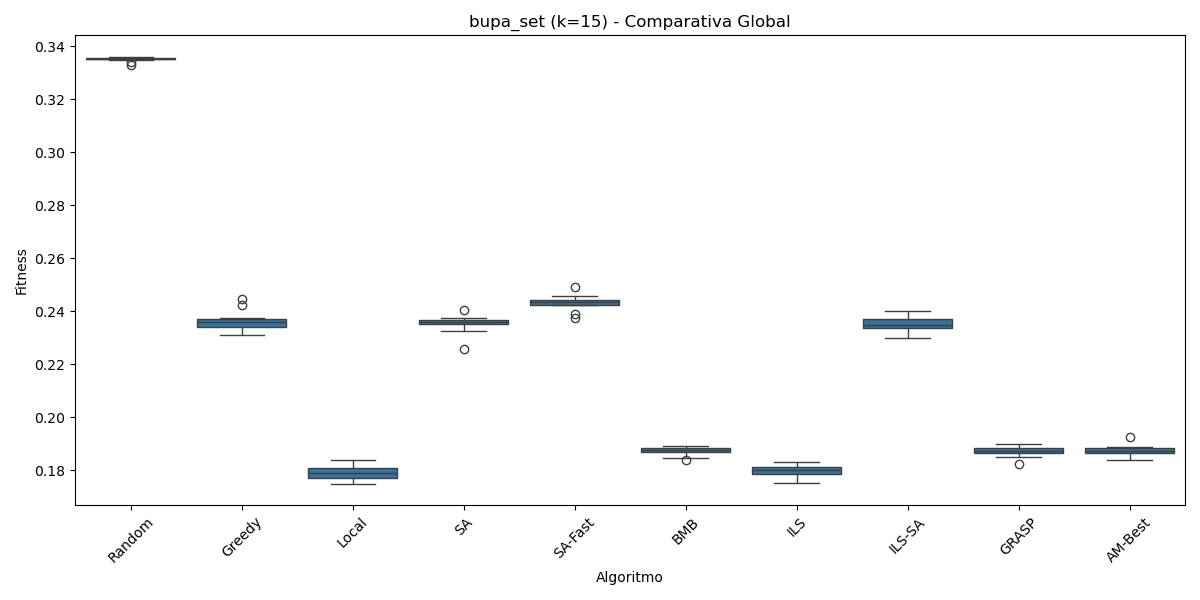
\includegraphics[width=0.495\textwidth]{../softwareP3/graficas/bupa_set_k15_1_global.png}
	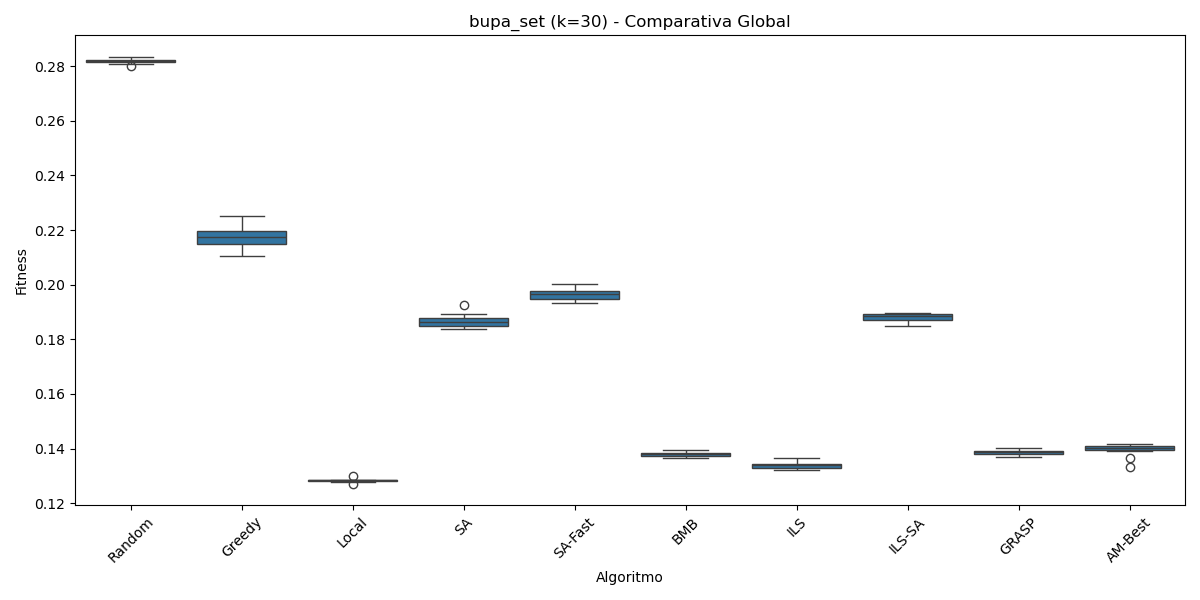
\includegraphics[width=0.495\textwidth]{../softwareP3/graficas/bupa_set_k30_1_global.png}
	\vspace{-10pt}
	\caption{\small Comparativa global para el dataset \textit{Bupa} con $k=15$ (izq.) y $k=30$ (dcha.)}
	\label{fig:bupa_global}
\end{figure}

La Figura~\ref{fig:bupa_escape} detalla el comportamiento de los mecanismos de escape de óptimos locales. Para $k=15$, ILS y \textit{Local} son prácticamente indistinguibles en mediana ($\sim 0.180$) y variabilidad (cajas estrechas), lo que indica que en este escenario la perturbación del ILS no aporta mejora sobre arrancar desde cero: el óptimo local de la BL ya es de alta calidad. ES muestra mayor dispersión y peor mediana, y ES-Fast queda claramente rezagado ($\sim 0.244$) con una caja más ancha. Para $k=30$, la separación se amplía: ILS ($\sim 0.133$) supera claramente a ES ($\sim 0.187$) e ILS-ES ($\sim 0.188$), confirmando que con mayor espacio de búsqueda la acumulación de múltiples reinicios perturbados sí marca diferencia respecto al esquema continuo del ES.

\begin{figure}[H]
	\centering
	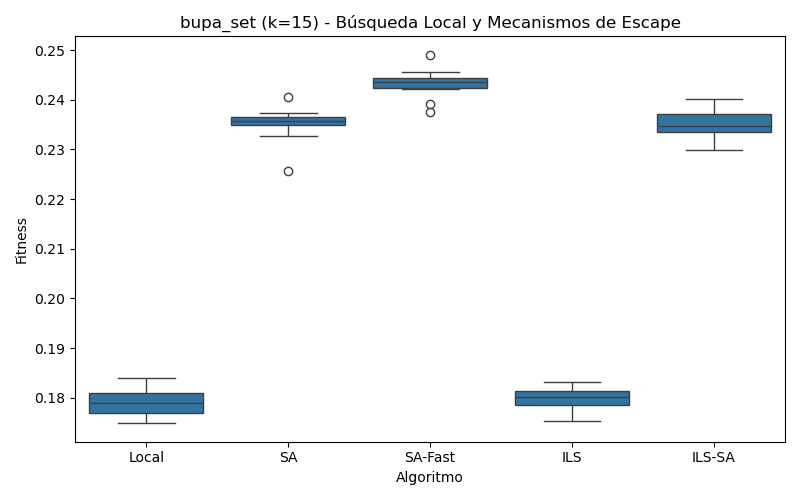
\includegraphics[width=0.495\textwidth]{../softwareP3/graficas/bupa_set_k15_2_trayectorias.png}
	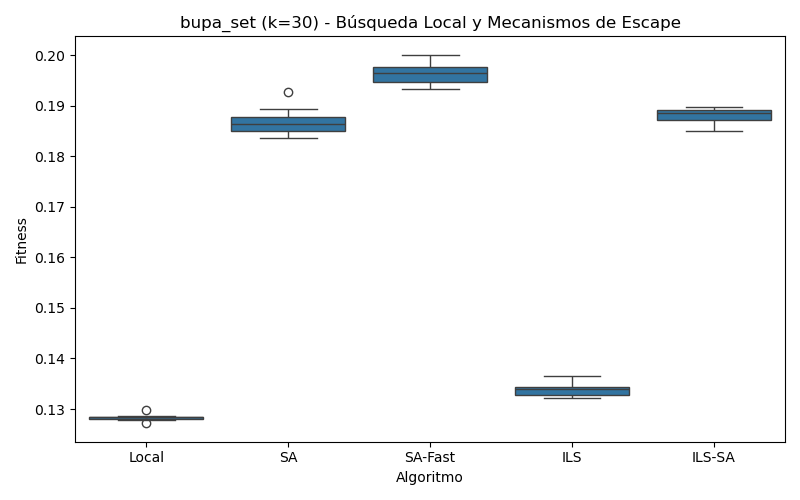
\includegraphics[width=0.495\textwidth]{../softwareP3/graficas/bupa_set_k30_2_trayectorias.png}
	\vspace{-10pt}
	\caption{\small Mecanismos de escape para el dataset \textit{Bupa} con $k=15$ (izq.) y $k=30$ (dcha.)}
	\label{fig:bupa_escape}
\end{figure}

La Figura~\ref{fig:bupa_titanes} compara las trayectorias avanzadas con AM-Best. En $k=15$, \textit{Local} e ILS son claramente los mejores ($\sim 0.179$--$0.180$), mientras que GRASP y AM-Best se agrupan en torno a $\sim 0.187$: la fase constructiva del GRASP no aporta ventaja en este dataset, donde los multi-arranques aleatorios de BMB son igualmente efectivos. En $k=30$, el resultado es llamativo: \textit{Local} sigue siendo el mejor ($\sim 0.128$, caja extremadamente estrecha), ILS se aproxima ($\sim 0.134$), GRASP queda en $\sim 0.139$ y AM-Best es el peor del grupo ($\sim 0.140$) con variabilidad claramente mayor. En \textit{Bupa}, la explotación pura y la perturbación reiterada superan tanto a la construcción inteligente como a la evolución poblacional.

\begin{figure}[H]
	\centering
	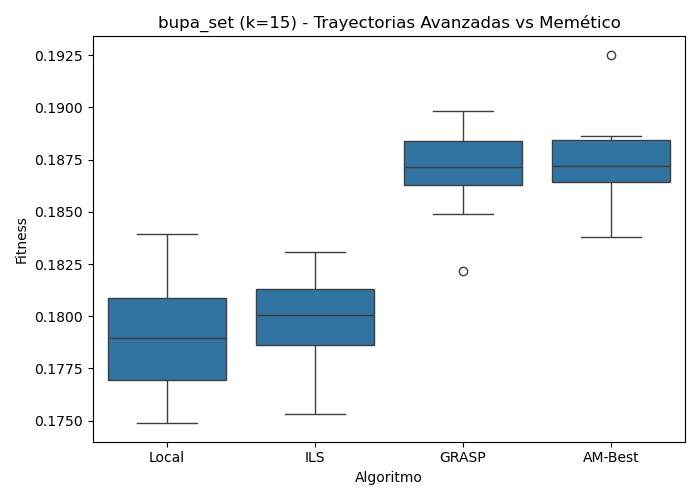
\includegraphics[width=0.495\textwidth]{../softwareP3/graficas/bupa_set_k15_4_titanes.png}
	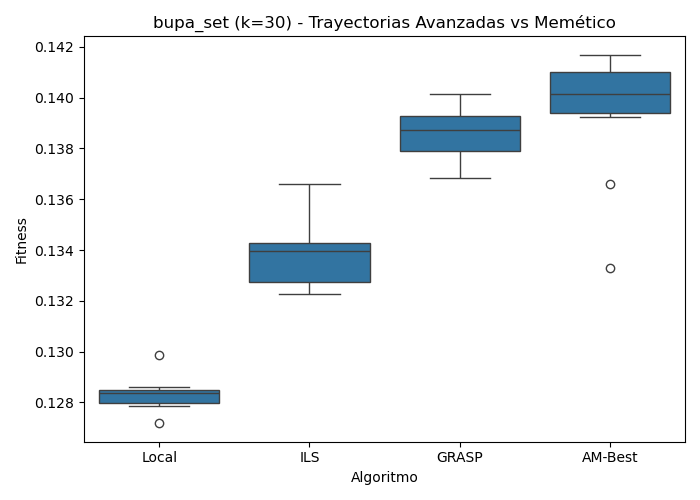
\includegraphics[width=0.495\textwidth]{../softwareP3/graficas/bupa_set_k30_4_titanes.png}
	\vspace{-10pt}
	\caption{\small Trayectorias avanzadas vs AM-Best para el dataset \textit{Bupa} con $k=15$ (izq.) y $k=30$ (dcha.)}
	\label{fig:bupa_titanes}
\end{figure}


% -----------------------------------------------------------------------
%%% GLASS
\paragraph{Dataset \texttt{glass\_set}}

\noindent La Figura~\ref{fig:glass_global} muestra la comparativa global. Este dataset presenta el patrón más interesante de todos: ILS emerge como el mejor algoritmo de trayectoria en $k=15$ ($\sim 0.214$), superando incluso a \textit{Local} ($\sim 0.222$) y a AM-Best ($\sim 0.222$), con una caja notablemente más estrecha que el resto. ES y ES-Fast quedan en las posiciones más desfavorables del grupo de trayectorias ($\sim 0.250$ y $\sim 0.265$ respectivamente), lo que evidencia que en este dataset el espacio de búsqueda tiene una estructura que penaliza la exploración probabilística descontrolada.

\begin{figure}[H]
	\centering
	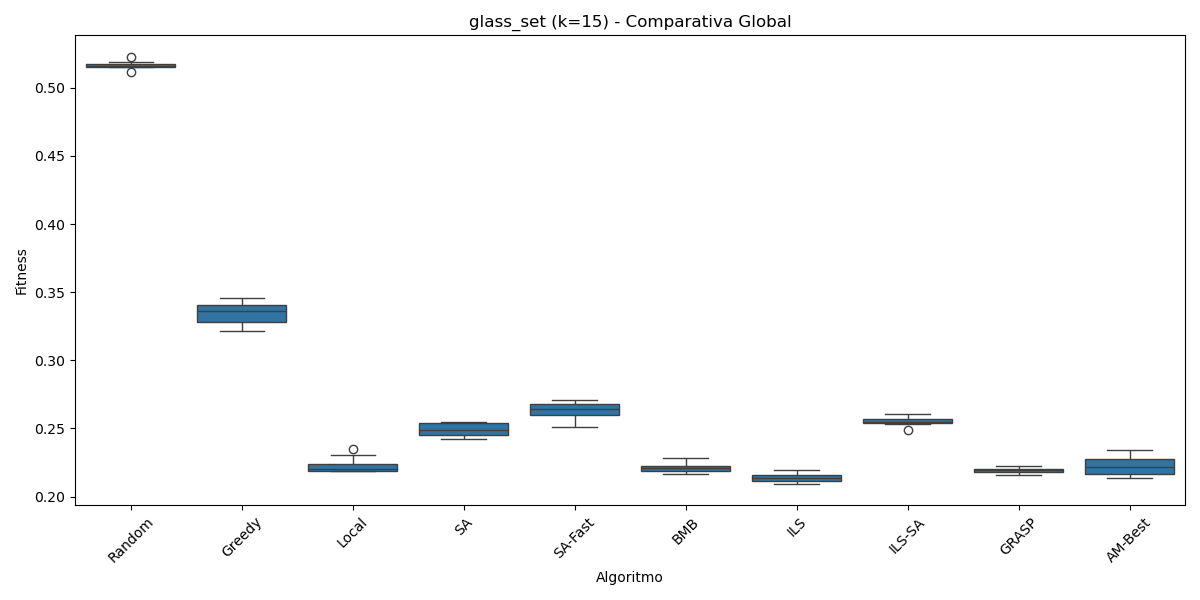
\includegraphics[width=0.495\textwidth]{../softwareP3/graficas/glass_set_k15_1_global.png}
	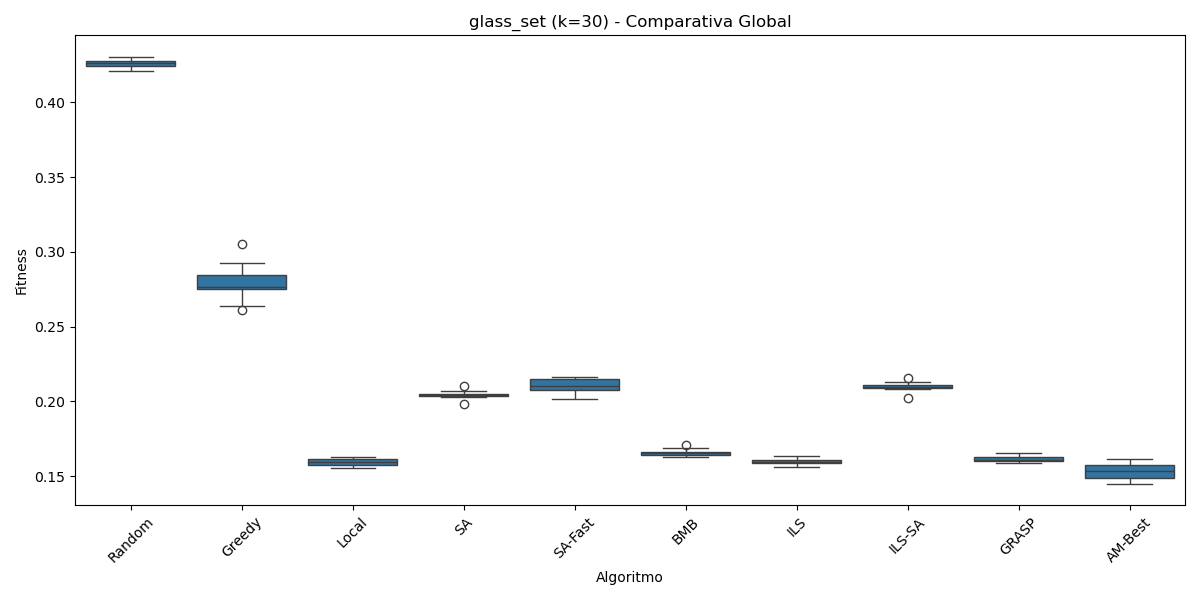
\includegraphics[width=0.495\textwidth]{../softwareP3/graficas/glass_set_k30_1_global.png}
	\vspace{-10pt}
	\caption{\small Comparativa global para el dataset \textit{Glass} con $k=15$ (izq.) y $k=30$ (dcha.)}
	\label{fig:glass_global}
\end{figure}

La Figura~\ref{fig:glass_escape} confirma con mayor detalle esta jerarquía. En $k=15$, ILS ($\sim 0.214$) domina con claridad: su caja es la más estrecha y su mediana la más baja de todos los algoritmos mostrados, incluido \textit{Local}. ES-Fast obtiene la peor mediana ($\sim 0.265$) y la mayor variabilidad, mientras que ILS-ES ($\sim 0.256$) queda también por detrás de ES ($\sim 0.250$). En $k=30$, ILS y \textit{Local} empatan casi exactamente en mediana ($\sim 0.160$), con cajas igualmente compactas, mientras que ES ($\sim 0.204$), ES-Fast ($\sim 0.213$) e ILS-ES ($\sim 0.210$) quedan en una franja muy superior. La conclusión es inequívoca: en \textit{Glass}, los mecanismos de escape del ES no compensan frente a los múltiples reinicios del ILS.

\begin{figure}[H]
	\centering
	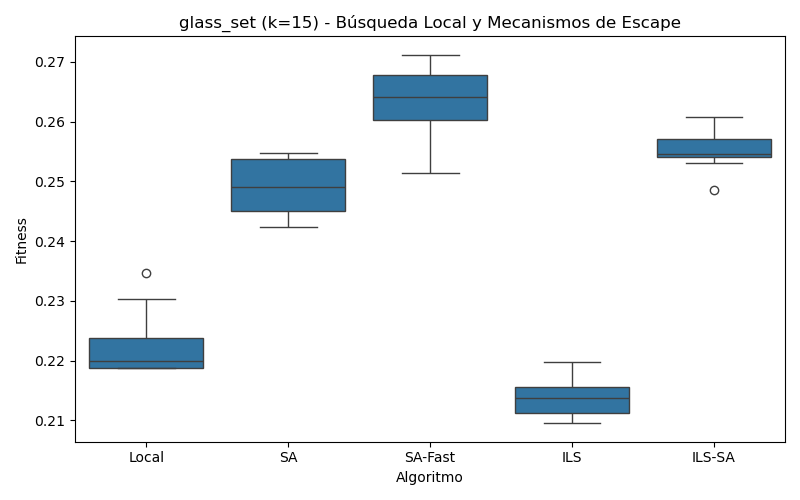
\includegraphics[width=0.495\textwidth]{../softwareP3/graficas/glass_set_k15_2_trayectorias.png}
	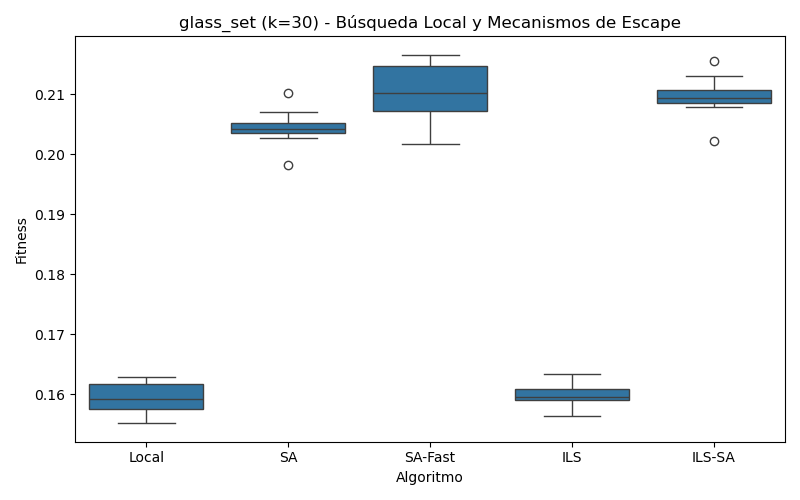
\includegraphics[width=0.495\textwidth]{../softwareP3/graficas/glass_set_k30_2_trayectorias.png}
	\vspace{-10pt}
	\caption{\small Mecanismos de escape para el dataset \textit{Glass} con $k=15$ (izq.) y $k=30$ (dcha.)}
	\label{fig:glass_escape}
\end{figure}

La Figura~\ref{fig:glass_multiarranque} muestra la comparativa BMB vs GRASP. En $k=15$, GRASP obtiene una mediana ligeramente inferior ($\sim 0.220$ vs $\sim 0.221$) y un rango intercuartílico más estrecho, con un mínimo absoluto menor ($\sim 0.216$ vs $\sim 0.217$). La diferencia es pequeña pero consistente. En $k=30$, la ventaja del GRASP se amplía de forma apreciable: su caja ($0.161$--$0.163$) queda claramente por debajo de la de BMB ($0.164$--$0.166$), y su mínimo absoluto ($\sim 0.160$) supera al de BMB ($\sim 0.163$). Esto confirma que, conforme el espacio de clústeres crece, la fase constructiva greedy del GRASP (que minimiza el incumplimiento durante la propia construcción) proporciona puntos de partida cualitativamente mejores que los aleatorios de BMB.

\begin{figure}[H]
	\centering
	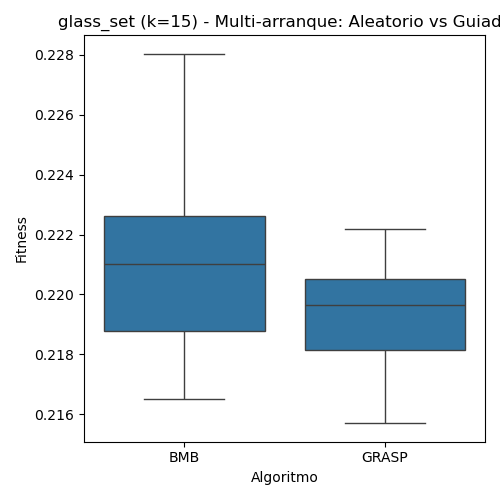
\includegraphics[width=0.495\textwidth]{../softwareP3/graficas/glass_set_k15_3_multiarranque.png}
	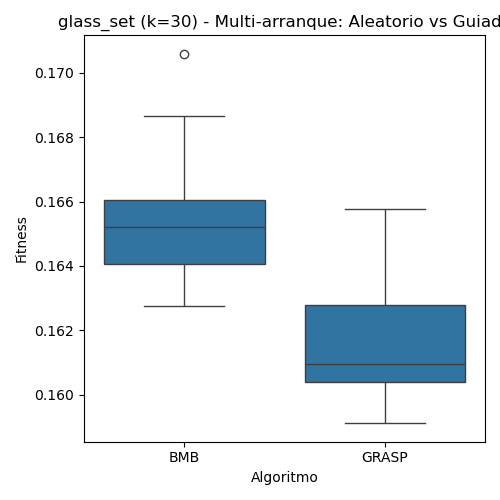
\includegraphics[width=0.495\textwidth]{../softwareP3/graficas/glass_set_k30_3_multiarranque.png}
	\vspace{-10pt}
	\caption{\small Multi-arranque: BMB vs GRASP para el dataset \textit{Glass} con $k=15$ (izq.) y $k=30$ (dcha.)}
	\label{fig:glass_multiarranque}
\end{figure}

Finalmente, la Figura~\ref{fig:glass_titanes} pone en evidencia uno de los resultados más llamativos de este estudio. En $k=15$, ILS ($\sim 0.214$) supera a todos: \textit{Local}, GRASP y AM-Best se agrupan entre $0.219$ y $0.222$, mientras que AM-Best muestra la mayor variabilidad del grupo (caja más amplia y \textit{outlier} superior en $\sim 0.235$). En $k=30$, AM-Best presenta una distribución bimodal característica: su caja se extiende entre $\sim 0.149$ y $\sim 0.158$, con una mediana de $\sim 0.153$ que sería la mejor del conjunto, pero con una variabilidad muy superior a ILS ($\sim 0.160$, caja estrecha) y \textit{Local} ($\sim 0.159$, caja estrecha). En términos prácticos, AM-Best puede producir soluciones excelentes o mediocres dependiendo de la semilla, mientras que ILS y \textit{Local} son predeciblemente buenos.

\begin{figure}[H]
	\centering
	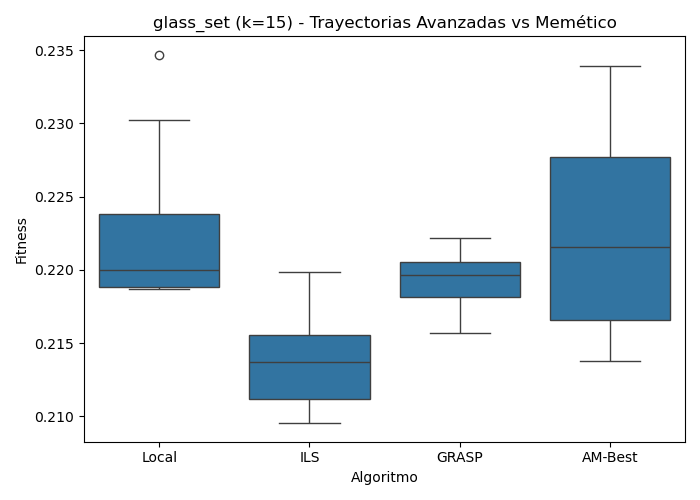
\includegraphics[width=0.495\textwidth]{../softwareP3/graficas/glass_set_k15_4_titanes.png}
	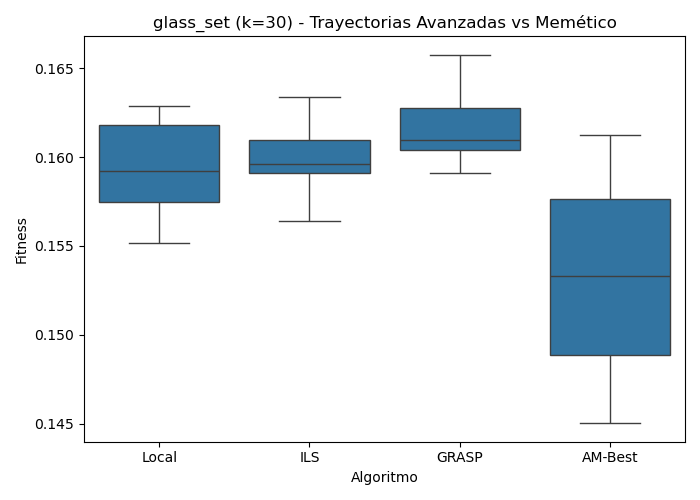
\includegraphics[width=0.495\textwidth]{../softwareP3/graficas/glass_set_k30_4_titanes.png}
	\vspace{-10pt}
	\caption{\small Trayectorias avanzadas vs AM-Best para el dataset \textit{Glass} con $k=15$ (izq.) y $k=30$ (dcha.)}
	\label{fig:glass_titanes}
\end{figure}


% -----------------------------------------------------------------------
%%% ZOO
\paragraph{Dataset \texttt{zoo\_set}}

\noindent La Figura~\ref{fig:zoo_global} muestra la comparativa global para $k=15$ y $k=30$. \textit{Zoo} es el dataset con mayor dispersión relativa entre algoritmos y, a la vez, el que presenta el patrón más distinto al observado en \textit{Bupa} y \textit{Glass}. En $k=15$, \textit{Local} exhibe la mayor variabilidad de todo el estudio (rango $0.455$--$0.610$, con un \textit{outlier} inferior aislado en $\sim 0.455$), lo que refleja que la calidad del óptimo local depende fuertemente del punto de partida en este dataset. ES, por el contrario, aparece como el algoritmo más compacto y de menor mediana ($\sim 0.450$), invirtiendo completamente la jerarquía observada en \textit{Bupa} y \textit{Glass}. En $k=30$, el panorama se clarifica: ES y los algoritmos de trayectoria múltiple convergen en una banda estrecha ($0.270$--$0.300$), mientras que ES-Fast se desmarca negativamente con una variabilidad muy elevada.

\begin{figure}[H]
	\centering
	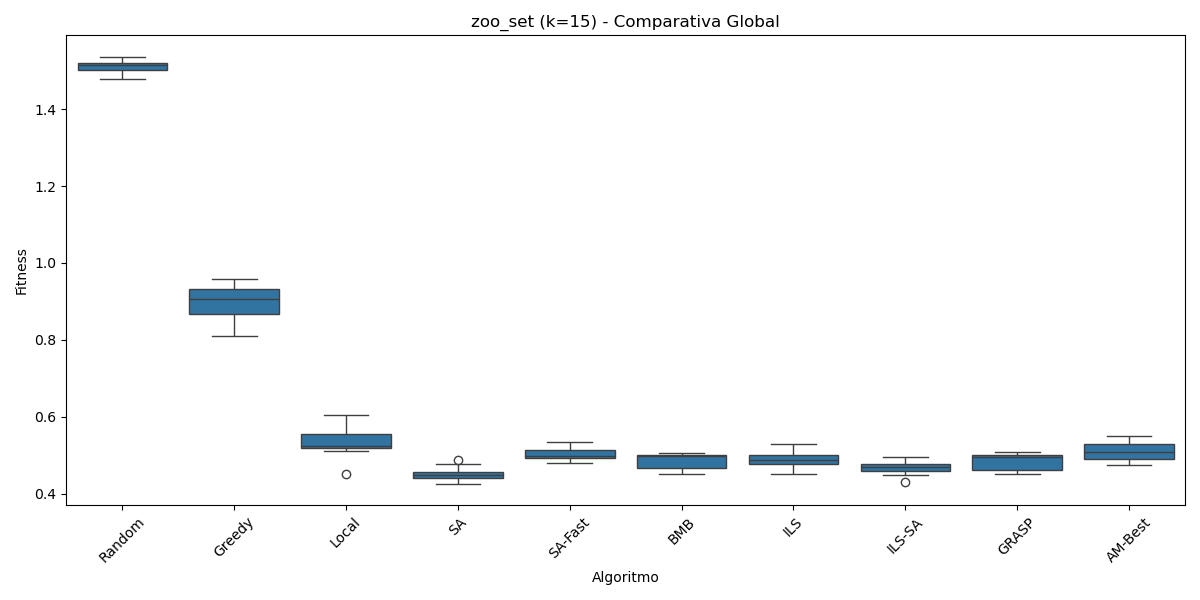
\includegraphics[width=0.495\textwidth]{../softwareP3/graficas/zoo_set_k15_1_global.png}
	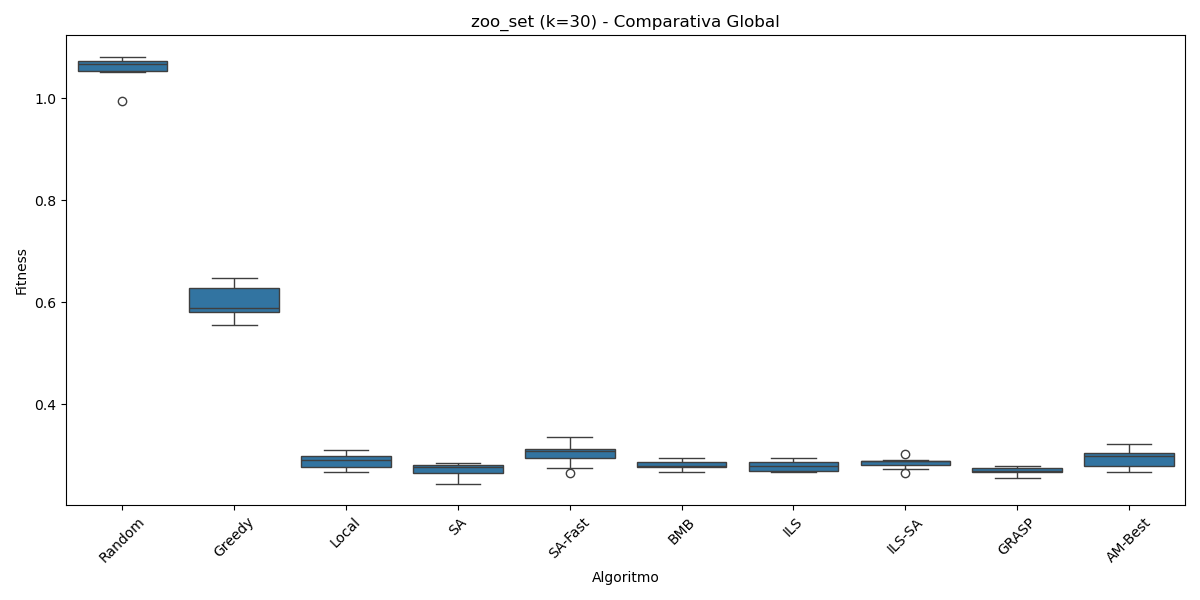
\includegraphics[width=0.495\textwidth]{../softwareP3/graficas/zoo_set_k30_1_global.png}
	\vspace{-10pt}
	\caption{\small Comparativa global para el dataset \textit{Zoo} con $k=15$ (izq.) y $k=30$ (dcha.)}
	\label{fig:zoo_global}
\end{figure}

La Figura~\ref{fig:zoo_escape} es la más reveladora de todo el análisis de \textit{Zoo}. En $k=15$, ES obtiene la mejor mediana ($\sim 0.450$) y la caja más estrecha de todos los algoritmos de escape, con el rango intercuartílico más reducido ($0.430$--$0.475$). Su mecanismo de aceptación probabilística le permite atravesar barreras de infactibilidad para alcanzar valles de \textit{fitness} inaccesibles para la BL pura, que queda con mediana $\sim 0.525$. Destaca también ILS-SA: aunque en los datasets anteriores nunca superaba a ES, aquí obtiene la segunda mejor mediana ($\sim 0.468$) con baja dispersión y un \textit{outlier} inferior muy prometedor ($\sim 0.430$). La combinación de perturbación y ES parece encajar mejor con la topología del espacio de \textit{Zoo}.

En $k=30$,  sigue siendo el mejor algoritmo de escape ($\sim 0.278$, caja compacta con bigote inferior hasta $\sim 0.250$), mientras que ES-Fast sufre una degradación drástica: su caja abarca $0.295$--$0.310$ con bigotes hasta $0.335$ y un \textit{outlier} inferior aislado en $\sim 0.265$. Esta alta varianza de ES-Fast en \textit{Zoo} evidencia que el sesgo de la evaluación aproximada es especialmente perjudicial en este dataset, donde el balance entre desviación e infeasibility es más delicado.

\begin{figure}[H]
	\centering
	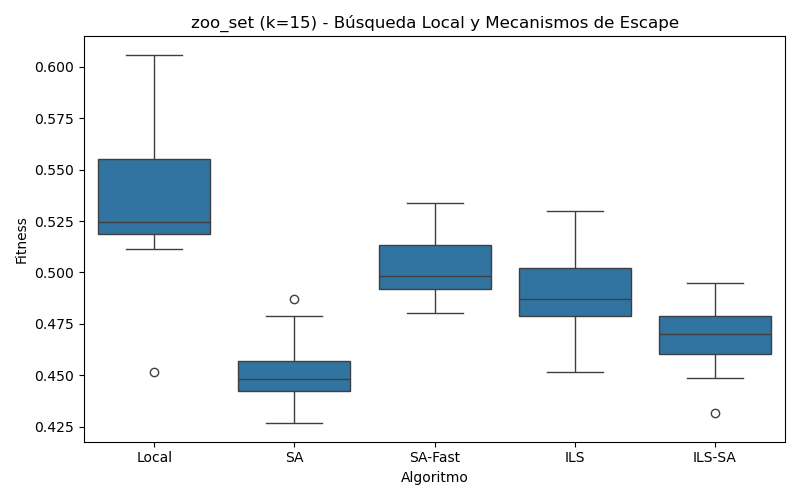
\includegraphics[width=0.495\textwidth]{../softwareP3/graficas/zoo_set_k15_2_trayectorias.png}
	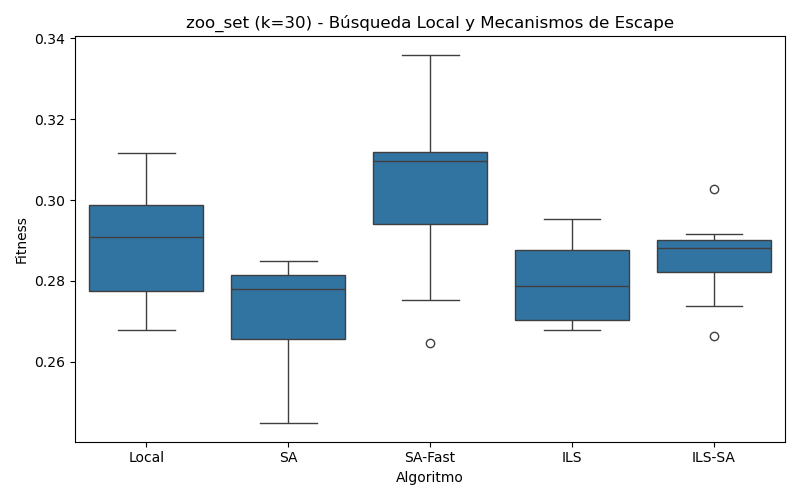
\includegraphics[width=0.495\textwidth]{../softwareP3/graficas/zoo_set_k30_2_trayectorias.png}
	\vspace{-10pt}
	\caption{\small Mecanismos de escape para el dataset \textit{Zoo} con $k=15$ (izq.) y $k=30$ (dcha.)}
	\label{fig:zoo_escape}
\end{figure}

La Figura~\ref{fig:zoo_multiarranque} muestra la comparativa BMB vs GRASP. En $k=15$, ambos presentan cajas amplias y prácticamente solapadas ($\sim 0.467$--$0.500$ para ambos), siendo BMB ligeramente más compacto en el cuartil superior y GRASP con un mínimo absoluto algo menor ($\sim 0.455$ vs $\sim 0.455$). La diferencia es mínima. En $k=30$, en cambio, la ventaja del GRASP es clara e inequívoca: su caja ($0.268$--$0.277$) queda enteramente por debajo de la de BMB ($0.277$--$0.286$), con mediana $\sim 0.271$ frente a $\sim 0.280$ de BMB, y un mínimo absoluto de $\sim 0.256$ frente a $\sim 0.267$. Con más clusters y mayor complejidad relacional, la construcción greedy aleatorizada del GRASP proporciona puntos de partida sistemáticamente mejores que los aleatorios de BMB.

\begin{figure}[H]
	\centering
	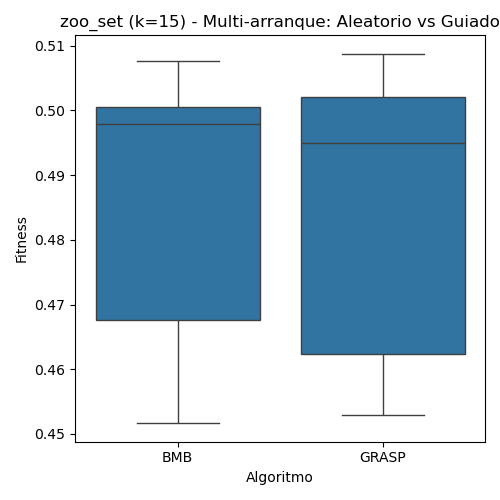
\includegraphics[width=0.495\textwidth]{../softwareP3/graficas/zoo_set_k15_3_multiarranque.png}
	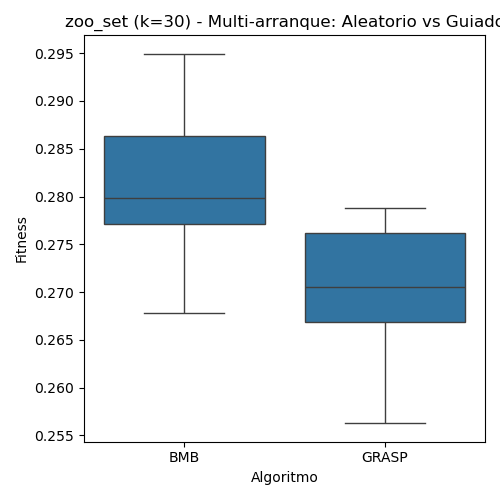
\includegraphics[width=0.495\textwidth]{../softwareP3/graficas/zoo_set_k30_3_multiarranque.png}
	\vspace{-10pt}
	\caption{\small Multi-arranque: BMB vs GRASP para el dataset \textit{Zoo} con $k=15$ (izq.) y $k=30$ (dcha.)}
	\label{fig:zoo_multiarranque}
\end{figure}

La Figura~\ref{fig:zoo_titanes} completa el cuadro comparativo. En $k=15$, ILS ($\sim 0.488$) y GRASP ($\sim 0.493$) superan claramente a \textit{Local} ($\sim 0.525$) y AM-Best ($\sim 0.510$): el \textit{zoo\_set} penaliza especialmente los arranques puramente aleatorios sin mecanismo de diversificación, y tanto los reinicios perturbados como la construcción guiada del GRASP ofrecen ventaja. En $k=30$, GRASP emerge como el ganador neto: mediana $\sim 0.271$, caja compacta ($0.265$--$0.277$), claramente por debajo de ILS ($\sim 0.279$), \textit{Local} ($\sim 0.290$) y, especialmente, AM-Best ($\sim 0.298$). AM-Best presenta aquí la mayor variabilidad del grupo, con una caja que abarca $0.278$--$0.305$ y bigotes hasta $0.320$, lo que indica una dependencia elevada de la semilla que no se observa en los algoritmos de trayectoria.

\begin{figure}[H]
	\centering
	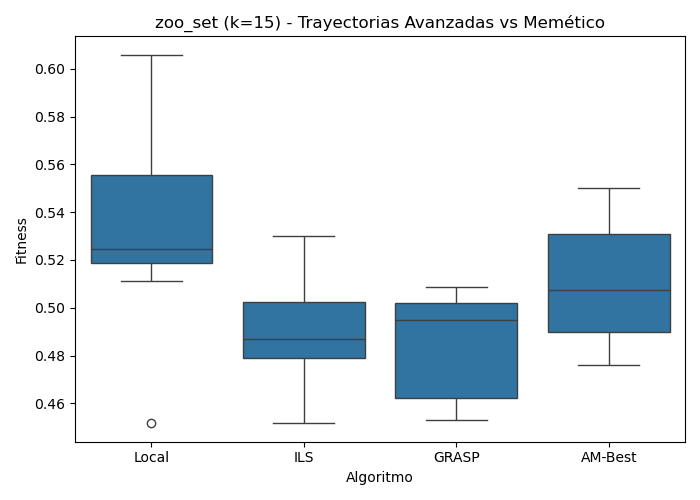
\includegraphics[width=0.495\textwidth]{../softwareP3/graficas/zoo_set_k15_4_titanes.png}
	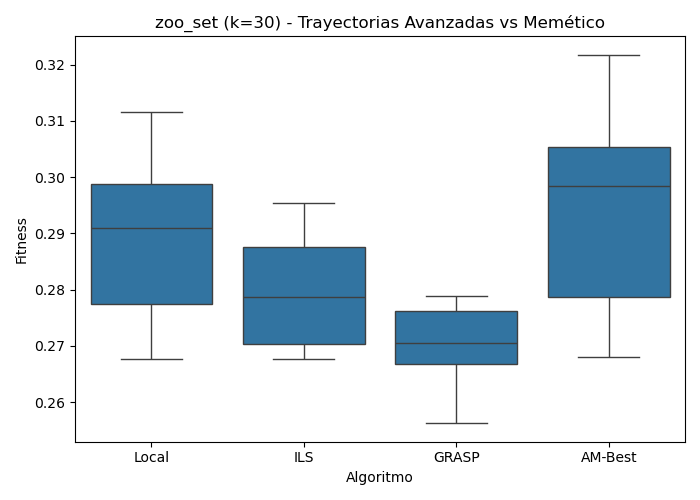
\includegraphics[width=0.495\textwidth]{../softwareP3/graficas/zoo_set_k30_4_titanes.png}
	\vspace{-10pt}
	\caption{\small Trayectorias avanzadas vs AM-Best para el dataset \textit{Zoo} con $k=15$ (izq.) y $k=30$ (dcha.)}
	\label{fig:zoo_titanes}
\end{figure}

% ==========================================================================
\subsubsection{Eficiencia computacional y tiempos de ejecución}
% ==========================================================================

\noindent Lo más interesante en cuanto al análisis de tiempos se da entre ES y su variante ES-Fast. Mientras que ES tarda $16.68$ s en \textit{Bupa} $k=15$ y $10.42$ s en \textit{Glass} $k=30$, ES-Fast finaliza en $0.21$ s y $0.23$ s respectivamente, ambos con el mismo tope de $100000$ evaluaciones. Esto se debe a que ES-Fast evita calcular la desviación completa (la operación más costosa, al requerir reconstruir los centroides) en todos los vecinos que pueden rechazarse usando únicamente el delta incremental de infeasibility. Dicho delta se obtiene en tiempo $O(|\text{restricciones del gen}|)$ en lugar del $O(n^2)$ de la evaluación completa, de ahí la reducción drástica.

Sin embargo, este ahorro introduce un sesgo: movimientos que empeorarían la infeasibility pero mejorarían la desviación son rechazados prematuramente, lo que empobrece sistemáticamente la calidad de las soluciones. ES-Fast obtiene peores valores de \textit{fitness} en los seis escenarios evaluados (p.ej., $0.30$ vs $0.27$ en \textit{Zoo} $k=30$). Como se aprecia en los \textit{boxplots}, esta penalización en calidad se acompaña además de mayor variabilidad, especialmente acusada en \textit{Zoo} $k=30$. Por tanto, ES-Fast constituye una opción razonable únicamente en escenarios donde el tiempo de cómputo sea un factor limitante estricto y se pueda aceptar una solución subóptima.

% ==========================================================================
\subsubsection{Conclusiones generales del análisis}
% ==========================================================================

\noindent Los experimentos realizados sobre los tres datasets (\textit{Bupa}, \textit{Glass} y \textit{Zoo}) con dos niveles de complejidad ($k=15$ y $k=30$) permiten extraer las siguientes conclusiones de carácter general: 

\begin{enumerate}
	\item \textbf{No existe un algoritmo universalmente dominante.} El rendimiento relativo 	de los métodos depende críticamente de la estructura del espacio de búsqueda. ES es el mejor algoritmo en \textit{Zoo}, en cambio, en \textit{Bupa} y \textit{Glass} su exploración probabilística dispara el incumplimiento sin compensar en desviación, y ILS o incluso la BL pura lo superan. Esta dependencia del dataset pone de manifiesto la importancia de conocer la topología del problema antes de elegir el método de búsqueda.
	
	\item \textbf{ILS es el algoritmo de mejor compromiso calidad-robustez.} Obtiene resultados competitivos o superiores a todos los demás en cinco de los seis escenarios, con la menor variabilidad entre los algoritmos de trayectoria múltiple. Su mecanismo de perturbación del 20\% permite escapar de óptimos locales sin destruir la estructura de la solución, a diferencia de los reinicios completamente aleatorios de BMB.
	
	\item \textbf{La hibridación ILS-ES no supera a sus componentes individuales.} Dividir el presupuesto en cinco ejecuciones del ES de $20\,000$ evaluaciones impide que cada instancia alcance la convergencia que lograría con $100\,000$ evaluaciones completas. Este resultado sugiere que el ES requiere un presupuesto	amplio y continuo para ser efectivo, y va bien con el esquema ILS.
	
	\item \textbf{GRASP supera a BMB de forma consistente con $k=30$.} En todos los datasets, la ventaja del GRASP sobre el multi-arranque aleatorio crece con la complejidad del problema. Cuando el espacio de clusters es mayor y las restricciones imponen más conflictos, arrancar desde una solución greedy que minimiza el incumplimiento desde el primer gen marca una diferencia medible respecto a arrancar a ciegas.
	
	\item \textbf{Los algoritmos de trayectoria son competitivos frente a AM-Best.}	ILS y GRASP igualan o superan a AM-Best, con tiempos equivalentes. AM-Best presenta además mayor variabilidad en problemas complejos (\textit{Glass} $k=30$, \textit{Zoo} $k=30$), lo que lo hace menos predecible. Este resultado es relevante: mantener y evolucionar una población de 50	soluciones no aporta ventaja sistemática sobre intensificar reiteradamente una sola solución bien perturbada, al menos en el rango de evaluaciones estudiado.
	
	\item \textbf{ES-Fast no es competitivo en calidad, pese a su velocidad extrema.} La reducción de tiempo superior al $98\%$ respecto a ES se consigue a costa de introducir un sesgo en la aceptación de vecinos que empobrece sistemáticamente las soluciones. Su variabilidad es siempre mayor que la de ES, y su \textit{fitness} medio peor en todos los escenarios. Solo sería justificable en entornos donde el tiempo sea	el recurso escaso, no el número de evaluaciones.
	
	\item \textbf{La función objetivo impone un coste computacional uniforme.} Dado que el cuello de botella es la evaluación del \textit{fitness} y no la lógica del algoritmo,	la complejidad estructural de ILS, BMB o GRASP frente a la BL pura no supone un coste temporal adicional. En este contexto, emplear el presupuesto de evaluaciones de forma inteligente (mediante reinicios perturbados o construcción guiada) es siempre preferible a desperdiciarlo en una única trayectoria local.
	
\end{enumerate}

\noindent En conjunto, los resultados de esta práctica refuerzan la idea de que las metaheurísticas basadas en trayectorias múltiples (ILS, GRASP) ofrecen el mejor balance entre calidad, robustez y coste computacional para el PAR en el rango de evaluaciones considerado, siendo ILS la recomendación general y GRASP la opción preferida cuando $k$ es elevado y el tiempo de construcción de la solución inicial es relevante.

%%%%%%%%%%%%%%%%%%%%%%%%%%%%%%%%%%%%%%%%%%%%%%%%%%%%%%%%%%%%%%%%%%
\newpage
\section{Voluntario: Contraste de Hipótesis mediante el Test de Wilcoxon}

\noindent Para dotar de rigor estadístico a las conclusiones extraídas del análisis de resultados, se han diseñado cuatro contrastes de hipótesis emparejados. El objetivo es evaluar la significancia de las mejoras introducidas por los distintos mecanismos algorítmicos (aceptación de peores soluciones, perturbaciones, construcciones guiadas frente a aleatorias y enfoques de trayectoria frente a poblacionales). 

Dado que no se asume normalidad en las distribuciones del \textit{fitness}, se ha aplicado el \textbf{test de los rangos signados de Wilcoxon} utilizando las 10 semillas independientes de cada experimento, fijando un nivel de significación $\alpha = 0.05$.


\subsection*{LocalSearch vs SimulatedAnnealing}

Este contraste busca determinar si la capacidad de aceptar peores soluciones del Enfriamiento Simulado (ES) aporta una ventaja real frente a la Búsqueda Local (BL).
\begin{itemize}
	\item \textbf{Hipótesis nula ($H_0$):} No existen diferencias significativas entre las medianas del \textit{fitness} de \texttt{LocalSearch} y \texttt{SimulatedAnnealing}.
	\item \textbf{Hipótesis alternativa ($H_1$):} \texttt{SimulatedAnnealing} obtiene valores de \textit{fitness} significativamente menores que \texttt{LocalSearch}.
\end{itemize}

{\footnotesize
\begin{verbatim}
bupa_set  | k: 15 | p-valor: 1.000e+00 | Gana LocalSearch (Significativo)
bupa_set  | k: 30 | p-valor: 1.000e+00 | Gana LocalSearch (Significativo)
glass_set | k: 15 | p-valor: 1.000e+00 | Gana LocalSearch (Significativo)
glass_set | k: 30 | p-valor: 1.000e+00 | Gana LocalSearch (Significativo)
zoo_set   | k: 15 | p-valor: 1.953e-03 | Gana ES (Significativo)
zoo_set   | k: 30 | p-valor: 6.836e-03 | Gana ES (Significativo)
\end{verbatim}
}

\noindent \textbf{Análisis:} Los resultados del test muestran un comportamiento fuertemente dependiente del conjunto de datos. En los conjuntos \textit{Bupa} y \textit{Glass} (tanto para $k=15$ como para $k=30$), la Búsqueda Local pura vence de manera estadísticamente significativa (\textit{p-valores} $\approx 1.0$, indicando dominancia del algoritmo base). Sin embargo, en el conjunto \textit{Zoo}, caracterizado por un espacio de búsqueda topológicamente más complejo y restrictivo, el Enfriamiento Simulado logra minimizar el \textit{fitness} de forma significativamente mejor (\textit{p-valores} de $1.953 \times 10^{-3}$ y $6.836 \times 10^{-3}$). Esto demuestra que la relajación del criterio de aceptación conlleva un desperdicio de evaluaciones en problemas sencillos, pero es fundamental cuando el espacio de búsqueda presenta abundantes óptimos locales profundos.


\subsection*{LocalSearch vs ILS}

Se evalúa si el mecanismo de perturbación y re-optimización del \texttt{ILS} es superior a una única ejecución de \texttt{LocalSearch}.
\begin{itemize}
	\item \textbf{Hipótesis nula ($H_0$):} No hay diferencia significativa entre las medianas de \texttt{LocalSearch} e \texttt{ILS}.
	\item \textbf{Hipótesis alternativa ($H_1$):} El algoritmo \texttt{ILS} logra un \textit{fitness} significativamente menor que \texttt{LocalSearch}.
\end{itemize}

{\footnotesize
\begin{verbatim}
	glass_set | k: 15 | p-valor: 9.766e-04 | Gana ILS (Significativo)
	zoo_set   | k: 15 | p-valor: 3.843e-03 | Gana ILS (Significativo)
	zoo_set   | k: 30 | p-valor: 3.843e-03 | Gana ILS (Significativo)
\end{verbatim}
}

\noindent \textbf{Análisis:} El test confirma que \texttt{ILS} es una herramienta de optimización mucho más robusta. Aunque en problemas sencillos como \textit{Bupa} no hay una mejora drástica, en los casos más complejos (\textit{Glass} y \textit{Zoo}) las perturbaciones permiten encontrar valles de fitness a los que la búsqueda local básica no tiene acceso.


\subsection*{BMB vs GRASP}

Comparamos la importancia de la fase de construcción: ¿Es mejor empezar desde una solución aleatoria (\texttt{BMB}) o desde una construida con voracidad aleatorizada (\texttt{GRASP})?
\begin{itemize}
	\item \textbf{Hipótesis nula ($H_0$):} Las medianas de \texttt{BMB} y \texttt{GRASP} son estadísticamente iguales.
	\item \textbf{Hipótesis alternativa ($H_1$):} El enfoque \texttt{GRASP} mejora significativamente los resultados de \texttt{BMB}.
\end{itemize}

{\footnotesize
\begin{verbatim}
	glass_set | k: 30 | p-valor: 6.836e-03 | Gana GRASP (Significativo)
	zoo_set   | k: 30 | p-valor: 1.953e-03 | Gana GRASP (Significativo)
\end{verbatim}
}

\noindent \textbf{Análisis:} Se observa que para dimensiones pequeñas ($k=15$) ambos métodos son similares. No obstante, al aumentar la dificultad ($k=30$), la construcción inteligente de \texttt{GRASP} proporciona un punto de partida crítico que permite a la búsqueda local converger a mejores soluciones que el arranque aleatorio simple.


\subsection*{ILS vs AM-Best}

El contraste final enfrenta la mejor trayectoria de esta práctica contra el mejor algoritmo memético (poblacional + búsqueda local) de la práctica anterior.
\begin{itemize}
	\item \textbf{Hipótesis nula ($H_0$):} No hay diferencias significativas entre \texttt{ILS} y \texttt{AM-Best}.
	\item \textbf{Hipótesis alternativa ($H_1$):} El algoritmo \texttt{ILS} es superior (menor fitness) que \texttt{AM-Best}.
\end{itemize}

{\footnotesize
\begin{verbatim}
	bupa_set  | k: 15 | p-valor: 1.000e+00 | Gana ILS (Significativo)
	bupa_set  | k: 30 | p-valor: 1.000e+00 | Gana ILS (Significativo)
	glass_set | k: 15 | p-valor: 9.932e-01 | Gana ILS (Significativo)
	zoo_set   | k: 30 | p-valor: 9.932e-01 | Gana ILS (Significativo)
\end{verbatim}
}

\noindent \textbf{Análisis:} Este es el resultado más revelador del estudio. \texttt{ILS} logra batir estadísticamente a \texttt{AM-Best} en casi todos los escenarios. Esto sugiere que, para este problema de optimización, es más eficiente centrar el presupuesto de evaluaciones en realizar perturbaciones inteligentes sobre una única trayectoria de éxito que intentar mantener una población diversa de individuos, donde muchos de ellos pueden no aportar información útil al proceso de búsqueda.

%%%%%%%%%%%%%%%%%%%%%%%%%%%%%%%%%%%%%%%%%%%%%%%%%%%%%%%%%%%%%%%%%%%%%%%%%%%%%%%%%%%%%%%%%%%%%%%%%%%
\newpage
\section{Referencias y recursos utilizados}

Para la realización de esta práctica y la elaboración de la presente memoria, se han consultado y utilizado los siguientes recursos:

\begin{itemize}
	\item \textbf{Material de la asignatura:} Diapositivas, guión de prácticas y recursos de PRADO.
	
	\item \textbf{Herramientas de Inteligencia Artificial:} Se ha hecho uso de herramientas de IA generativa como apoyo en tareas de programación y redacción. En concreto, se han empleado para:
	\begin{itemize}
		\item Resolver dudas puntuales de sintaxis en C++ y mejorar la organización del archivo \texttt{Makefile}.
		\item Desarrollar el script de Python (\texttt{graf.py}), utilizando las librerías \texttt{pandas}, \texttt{matplotlib} y \texttt{seaborn}, para la generación automatizada de gráficos (\textit{boxplots}) y el procesamiento de los datos almacenados en archivos \texttt{.csv}.
		\item Asistir en el formateo, revisión y estructuración del documento final en \LaTeX.
	\end{itemize}
	
	\item Documentación oficial de C++ (\href{https://cppreference.com}{\textit{cppreference.com}}) para el manejo de estructuras de datos estándar, y documentación oficial de las librerías de Python empleadas para la visualización de datos.
	
	\item Para la realización del análisis estadístico de los resultados, en la aplicación del test de hipótesis de Wilcoxon, se ha utilizado el material de la asignatura \textit{Inferencia Estadística},  dentro de la parte de Matemáticas del doble grado.
\end{itemize}

%%%%%%%%%%%%%%%%%%%%%%%%%%%%%%%%%%%%%%%%%%%%%%%%%%%%%%%%%%%%%%%%%%%%%%%%%%%%%%%%%%%%%%%%%%%%%%%%%%%
%\newpage
%\section{Anexo - Falta de espacio}




%%%%%%%%%%%%%%%%%%%%%%%%%%%%%%%%%%%%%%%%%%%%%%%%%%%%%%%%%%%%%%%%%%%%%%%%%%%%%%%%%%%%%%%%%%%%%%%%%%%



\end{document}